\documentclass[twoside]{article}
\author{Michele Mazza}
% Pacchetti di Codifica e Lingua
\usepackage[utf8]{inputenc}
\usepackage[T1]{fontenc}
\usepackage[italian]{babel}

% Pacchetti Grafici e Diagrammi
\usepackage{graphicx}
\usepackage{tikz}
\usepackage{tikz-3dplot}
\usetikzlibrary{angles,quotes,arrows.meta, positioning, 3d, matrix, calc}
\usepackage{pgfplots}
\pgfplotsset{compat=1.18}

% Pacchetti Matematici
\usepackage{amsmath, amssymb}

% Scegliere tra amsthm e ntheorem
%\usepackage{ntheorem}
% Se si preferisce amsthm, commentare la riga sopra e decommentare la seguente
\usepackage{amsthm}
\usepackage{cancel}

% Pacchetti per Tabelle e Unità di Misura
\usepackage{geometry}
\usepackage{siunitx}
\usepackage{booktabs}
\usepackage{tabularx}
\usepackage{colortbl}
\usepackage{adjustbox}

% Pacchetti per Layout e Formattazione
\usepackage{fancyhdr}
\usepackage{float}
\usepackage{microtype}
\usepackage{multicol}

% Altri Pacchetti Utili
\usepackage{mdframed}
\usepackage{animate}
\usepackage{ulem}
\usepackage{eurosym}

% Pacchetto enumitem
\usepackage{enumitem}

% Definizioni dei Colori e Comandi Personalizzati
\definecolor{lightblue}{HTML}{9cd8fc}
\definecolor{myblue}{HTML}{139FE9}
\definecolor{myblack}{HTML}{303030}
\definecolor{mygray}{HTML}{787878}
\definecolor{mywhite}{HTML}{c7c7c7}
\newcommand{\norm}[1]{\left\lVert#1\right\rVert}

% Ambienti Personalizzati
% Usa \theoremstyle e \theorembodyfont come necessario
\newmdtheoremenv[
    backgroundcolor=orange!10,
    linecolor=myblue,
    linewidth=0pt,
    leftmargin=0pt,
    rightmargin=0pt,
    innerleftmargin=10pt,
    innerrightmargin=10pt,
    innertopmargin=10pt,
    innerbottommargin=10pt,
    nobreak
]{curiosity}{Curiosità}

\newmdtheoremenv[
    font=\normalfont\small,
    linewidth=0pt,
    innerleftmargin=10pt,
    innerrightmargin=10pt,
]{example}{Esempio}

\newmdtheoremenv[
  backgroundcolor=lightblue,
  linecolor=myblue,
  linewidth=1.5pt,
  innertopmargin=10pt,
  innerbottommargin=10pt,
  innerrightmargin=10pt,
  innerleftmargin=10pt,
  nobreak
]{theorem}{Teorema}

\newmdtheoremenv[
  backgroundcolor=gray!10,
  linewidth=0pt,
  innertopmargin=-5pt,
  innerbottommargin=5pt,
  innerrightmargin=10pt,
  innerleftmargin=10pt,
  nobreak
]{definition}{Definizione}

\newmdtheoremenv[
  backgroundcolor=gray!10,
  linecolor=myblue,
  linewidth=1.5pt,
  innertopmargin=-5pt,
  innerbottommargin=5pt,
  innerrightmargin=10pt,
  innerleftmargin=10pt,
  nobreak
]{proposition}{Proposizione}


% Configurazioni di fancyhdr
\pagestyle{fancy}
\fancyhf{}
\fancyhead[RE,RO]{\nouppercase{\rightmark}}
\fancyfoot[C]{\thepage}
\renewcommand{\headrulewidth}{0.0pt}
\renewcommand{\footrulewidth}{0pt}
\geometry{a4paper, left=20mm, right=20mm, top=20mm, bottom=20mm}

\usepackage{titlesec} % Pacchetto per personalizzare i titoli delle sezioni

% Definisci i colori per le diverse sezioni
\titleformat{\section}
{\color{black}\normalfont\Large\bfseries}
{\thesection}{1em}{}

\titleformat{\subsection}
{\color{red}\normalfont\large\bfseries}
{\thesubsection}{1em}{}

\titleformat{\subsubsection}
{\color{blue}\normalfont\normalsize\bfseries}
{\thesubsubsection}{1em}{}

% Pacchetti Aggiuntivi
\usepackage{xparse,array}

% Pacchetto Hyperref (inserito per ultimo)
\usepackage{hyperref}

\begin{document}
\title{Fisica Generale T-B Elettromagnetismo}
\maketitle
\hrulefill
\section{Introduzione, concetti matematici utili}
Si intendono scontati i concetti affrontati in \begin{itemize}
    \item Algebra e Geometria (Prof. Gimigliano)
    \item Analisi Matematica T-A (Prof. Cataldo)
    \item Fisica Generale T-A (Prof.ssa Bellini)
\end{itemize}
\subsection{Tipologie di funzioni}
\subsubsection{Funzioni scalari}
Sono le funzioni che vanno da $\mathbb{R}^n \to \mathbb{R}$, con $n \geq 1$.
\begin{itemize}
    \item $f: \mathbb{R} \to \mathbb{R}$
          \begin{figure}[H]
              \centering
              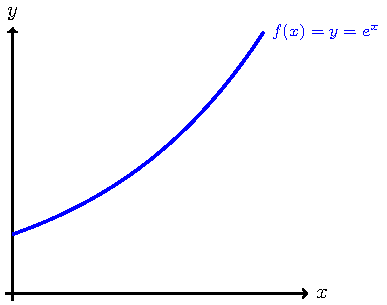
\includegraphics{src/functions/image2.pdf}
              \label{fig:funzioni2}
          \end{figure}
    \item $f: \mathbb{R}^2 \to \mathbb{R}$
          \begin{figure}[H]
              \centering
              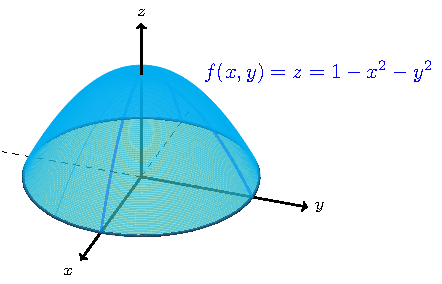
\includegraphics{src/functions/image1.pdf}
              \label{fig:funzioni3}
          \end{figure}
    \item $f: \mathbb{R}^3 \to \mathbb{R}$ non è rappresentabile graficamente, (si utilizzano gli insiemi di livello per rappresentarle, in pratica si fissa un valore di $f$ e si rappresenta la superficie che lo assume).
\end{itemize}
\subsubsection{Funzioni vettoriali}
Sono le funzioni che vanno da $\mathbb{R} \to \mathbb{R}^m$, con $n\geq 1$ e $m\geq 2$.
\begin{itemize}
    \item $f: \mathbb{R} \to \mathbb{R}^2$, le curve piane.

\end{itemize}
\section{Elettrostatica}
\subsection{Carica elettrica}
La carica elettrica è espressione di una proprietà intrinseca della materia ed è la grandezza fisica
responsabile delle interazioni elettriche. Le cariche elettriche possono essere positive (protoni) e
negative (elettroni). I corpi in natura sono generalmente neutri, ovvero hanno lo stesso numero di
cariche positive e negative; se un corpo è elettricamente carico può esserlo positivamente
(mancanza di elettroni) o negativamente (eccesso di elettroni).
\begin{figure}[H]
    \centering
    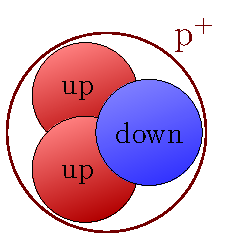
\includegraphics[width=0.15\textwidth]{src/atom/image1.pdf}
    \label{fig:carica1}
    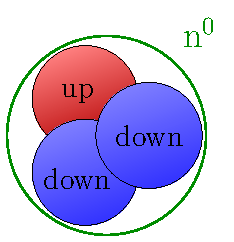
\includegraphics[width=0.15\textwidth]{src/atom/image2.pdf}
    \label{fig:carica2}
    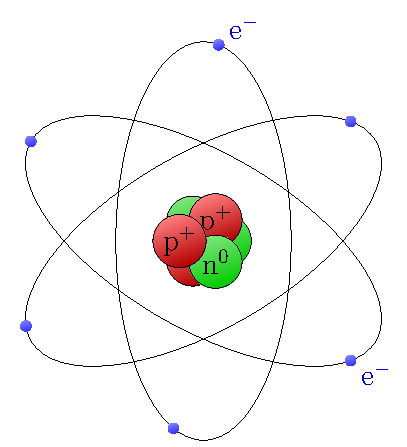
\includegraphics[width=0.2\textwidth]{src/atom/image3.pdf}
    \label{fig:carica3}
    \caption{Cariche elettriche}
\end{figure}
\subsubsection{Isolanti e conduttori}
I corpi macroscopici si possono suddividere in isolanti, nei quali la carica elettronica non è libera di
muoversi; conduttori, in cui gli elettroni (detti di conduzione) si possono muovere liberamente
attraverso il corpo, e semiconduttori, in cui le cariche si possono muovere sotto determinate
condizioni.
\begin{figure}[H]
    \centering
    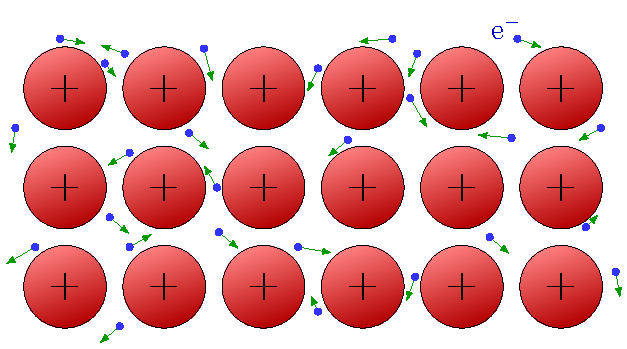
\includegraphics[width=0.2\textwidth]{src/atom/image4.pdf}
    \label{fig:carica4}
    \caption{Moto delle cariche elettriche in un conduttore}
\end{figure}
\subsubsection{Elettrizzazione per strofinio}
I corpi isolanti si possono caricare elettricamente per strofinio (triboelettricità),
acquistando o cedendo elettroni ad un altro corpo (a seconda della posizione relativa nella serie
triboelettrica). I conduttori si possono caricare elettricamente per strofinio solo se
opportunamente isolati dall’ambiente circostante.
\begin{figure}[H]
    \centering
    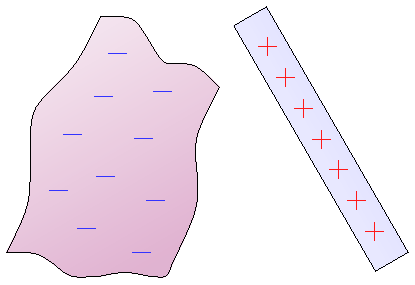
\includegraphics[width=0.25\textwidth]{src/charge/image1.pdf}
    \label{fig:charge1}
    \caption{Elettrizzazione per strofinio}
\end{figure}
\subsubsection{Importante}
Quando si carica o si scarica un corpo, l'unica cosa che si muove sono gli elettroni del livello più esterno non i protoni.
\begin{figure}[H]
    \centering
    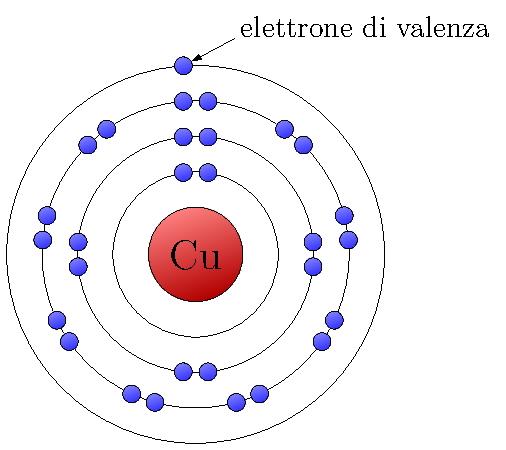
\includegraphics[width=0.25\textwidth]{src/atom/image5.pdf}
    \label{fig:carica5}
    \caption{Rappresentazione di livelli di valenza di un atomo}
\end{figure}
\subsubsection{Alcune costanti}
\begin{itemize}
    \item Il raggio medio dell'atomo è $r_{nucleo} = \SI{1e-10}{\meter}$.
    \item Il raggio del nucleo è $r_{atomo} = \SI{1e-15}{\meter}$.
    \item La carica elementare è $e = \SI{1.6e-19}{\coulomb}$.
    \item La carica del protone è $q_p = \SI{1.6e-19}{\coulomb}$.
    \item La carica dell'elettrone è $q_e = \SI{-1.6e-19}{\coulomb}$.
    \item La massa del protone è $m_p = \SI{1.67e-27}{\kilo\gram}$.
    \item La massa dell'elettrone è $m_e = \SI{9.11e-31}{\kilo\gram}$.
    \item La massa del neutrone è $m_n = \SI{1.67e-27}{\kilo\gram}$.
    \item La costante di Coulomb è $k = \SI{8.99e9}{\newton\square\meter\per\square\coulomb}$ e si calcola come $k = \displaystyle \frac{1}{4\pi\varepsilon_0}$.
    \item La costante dielettrica del vuoto è $\varepsilon_0 = \SI{8.85e-12}{\coulomb\square\per\newton\per\square\meter}$.
\end{itemize}

\subsection{Legge di Coulomb}
\subsubsection{Forza elettrostatica}
Il modulo della forza $F$ che si esercita tra due cariche puntiformi $q_1$ e $q_2$ poste a distanza $r$ nel vuoto
è data dalla forza di Coulomb:
\begin{equation}
    \boxed{\vec{F}_{12} = \displaystyle \frac{1}{4\pi\varepsilon_0} \cdot \frac{q_1q_2}{\left(r_{12}\right)^2}\cdot \hat{r}_{12}}
\end{equation}
dove $\hat{r}_{12} = \displaystyle \frac{\vec{r}_{12}}{|\vec{r}_{12}|}$ è il versore diretto da $q_1$ a $q_2$ e $r_{12}$ è la distanza tra le due cariche.
\begin{equation*}
    \boxed{F_{12} = \displaystyle \frac{1}{4\pi\varepsilon_0} \cdot \frac{q_1 q_2}{\left(r_{12}\right)^2}}
\end{equation*}
\begin{equation*}
    \boxed{F = \displaystyle \frac{|q_1| |q_2|}{4\pi\varepsilon_0 r^2}}
\end{equation*}
\begin{equation}
    \boxed{\vec{F}_{12} = \displaystyle k \cdot \frac{q_1 q_2}{\left(r_{12}\right)^2} \cdot \hat{r}_{12}}
\end{equation}
dove $k = \displaystyle \frac{1}{4\pi\varepsilon_0}$ è la costante di Coulomb.
\begin{figure}[H]
    \centering
    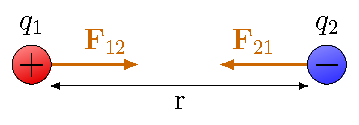
\includegraphics[width=0.3\textwidth]{src/coulomb/image5.pdf}
    \label{fig:coulomb5}\\
    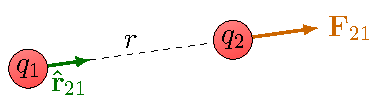
\includegraphics[width=0.35\textwidth]{src/coulomb/image1.pdf}
    \label{fig:coulomb1}
    \caption{Forza elettrostatica}
\end{figure}
\subsubsection{ATTENTO !}
Il prof usa la convenzione strana, utilizza $F_{12}$ e la applica su $q_1$ non su $q_2$, così come per il raggio $r_{12}$, lo applica su $q_2$ e non su $q_1$.
\subsubsection{Forza elettrostatica con più cariche}
Vale il \textbf{principio di sovrapposizione del campo elettrostatico}, per un sistema di $n$ cariche puntiformi:
\begin{equation}
    \boxed{\vec{F}_1 = \displaystyle \frac{q_{1}}{4 \pi \varepsilon_0} \sum_{i=2}^{n} \frac{q_{i}}{(r_{1i})^{2}} \hat{r}_{1i}}
\end{equation}
\begin{equation}
    \boxed{\vec{F}_1 = \displaystyle k q_1 \cdot \sum_{i=2}^{n} \frac{q_{i}}{(r_{1i})^{2}} \hat{r}_{1i}}
\end{equation}
\begin{figure}[H]
    \centering
    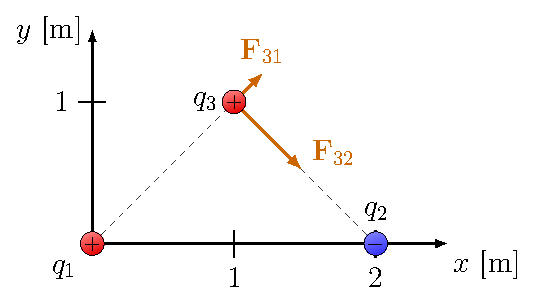
\includegraphics[width=0.35\textwidth]{src/coulomb/image6.pdf}
    \label{fig:coulomb6}
    \caption{Forza elettrostatica con più cariche}
\end{figure}

\subsection{Campo elettrostatico}
\subsubsection{Campo elettrostatico di una carica puntiforme}
In ogni punto $P$ dello spazio si può definire un \textbf{campo elettrostatico} $\vec{E}(P)$ come:\\
La forza, dovuta a tutte le cariche \textbf{sorgenti} presenti, agente su una \textbf{carica sonda} $q$ molto piccola (al limite, tendente a zero), divisa per la carica sonda stessa, ovvero la forza totale agente su una carica unitaria posta in $P$, a distanza $\vec{r}$ dalla carica sorgente $Q$:
\begin{equation}
    \boxed{\vec{E}(P)=\vec{E}(\vec{r}) = \displaystyle \frac{\vec{F}(\vec{r})}{q}}
\end{equation}
\begin{equation*}
    \vec{E}(\vec{r}) = \displaystyle \frac{1}{q} \cdot \left(\frac{1}{4\pi\varepsilon_0} \cdot \frac{q Q}{r^2} \cdot \hat{r}\right)
\end{equation*}
\begin{equation*}
    \vec{E}(\vec{r}) = \displaystyle \frac{1}{\cancel{q}} \cdot \left(\frac{1}{4\pi\varepsilon_0} \cdot \frac{\cancel{q} Q}{r^2} \cdot \hat{r}\right)
\end{equation*}
\begin{equation}
    \boxed{\vec{E}(\vec{r}) = \displaystyle \frac{1}{4\pi\varepsilon_0} \cdot \frac{Q}{r^2} \cdot \hat{r}}
\end{equation}
\begin{equation}
    \boxed{\vec{E}(\vec{r}) = \displaystyle k \cdot \frac{Q}{r^2} \cdot \hat{r}}
\end{equation}
\begin{itemize}
    \item Questa grandezza, come noti, è \textbf{indipendente} da $q$, ma solo dalla carica sorgente $Q$ e dalla posizione del punto $P$.
    \item Ha la \textbf{stessa direzione} e verso della forza di Coulomb $\vec{F}$
    \item \'E generato da $Q$.
\end{itemize}
\begin{figure}[H]
    \centering
    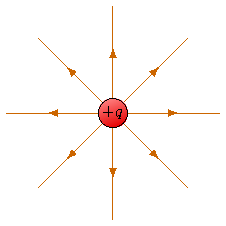
\includegraphics[width=0.25\textwidth]{src/electricfield/image1.pdf}
    \label{fig:electricfield1}
    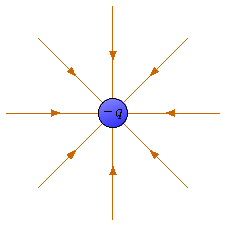
\includegraphics[width=0.25\textwidth]{src/electricfield/image2.pdf}
    \label{fig:electricfield2}
    \caption{Campo elettrostatico di una carica puntiforme}
\end{figure}
\subsubsection{Campo elettrostatico con limite}
A questo punto, si può definire il campo elettrostatico come:
\begin{equation}
    \boxed{\vec{E}(\vec{r}) = \lim_{q \to 0} \displaystyle \frac{\vec{F}(\vec{r})}{q}}
\end{equation}
è importante notare che $q$ non può "tendere" a zero, in quanto la carica va a multipli di $e$, è una quantità discreta, ma a livello matematico si può fare.
\subsubsection{Campo elettrostatico con più cariche}
Vale il \textbf{principio di sovrapposizione del campo elettrostatico}, per un sistema di $n$ cariche $Q_i$ puntiformi, in un punto $P$ dello spazio il campo elettrostatico totale è la somma vettoriale dei campi elettrici generati da ciascuna carica rispetto a $P$:
\begin{equation}
    \boxed{\vec{E}(P) = \displaystyle \sum_{i=1}^{n} \vec{E}_i(P)}
\end{equation}
\begin{equation}
    \boxed{\vec{E}(P) = \displaystyle \sum_{i=1}^{n} \displaystyle \frac{1}{4\pi\varepsilon_0} \cdot \frac{Q_i}{r_i^2} \cdot \hat{r}_i}
\end{equation}
\begin{figure}[H]
    \centering
    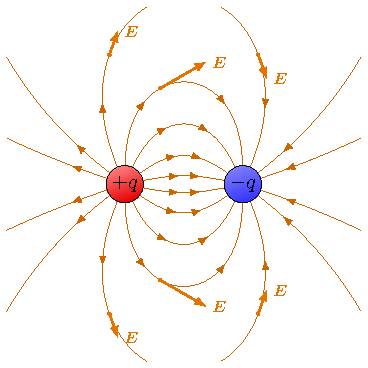
\includegraphics[width=0.3\textwidth]{src/electricfield/image4.pdf}
    \label{fig:electricfield4}
    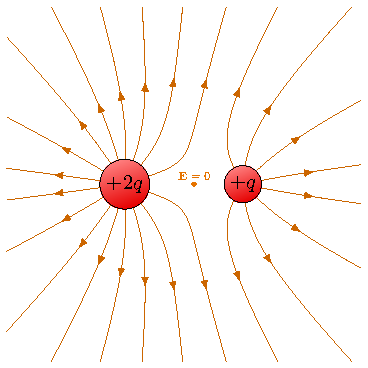
\includegraphics[width=0.3\textwidth]{src/electricfield/image6.pdf}
    \label{fig:electricfield6}
    \caption{Campo elettrostatico con più cariche}
\end{figure}
\newpage
\subsection{Campo elettrostatico di un sistema continuo di cariche}
Nel caso di distribuzione continua di carica (sorgente), la sommatoria è sostituita da un integrale vettoriale esteso a tutta la distribuzione di carica
\begin{equation}
    \boxed{\vec{E}= \displaystyle \int d \vec{E}}
\end{equation}
\begin{equation*}
    d \vec{E} = d E \cdot \hat{r}
\end{equation*}
\begin{equation*}
    d \vec{E} = \displaystyle \frac{1}{4\pi\varepsilon_0} \cdot \frac{dq}{r^2} \cdot \hat{r}
\end{equation*}
\begin{equation*}
    d E = \displaystyle k \cdot \frac{d q}{r^2} \cdot \hat{r}
\end{equation*}
ovvero il campo elettrostatico infinitesimo $dE$ è generato da un elemento di carica infinitesimo $dq$.\\
\'E utile ricavarsi $dq$ dalla densità di carica $\rho$:
\subsubsection{Campo elettrostatico di un filo carico}
Chiamiamo "lambda" la densità lineare di carica, ovvero la carica per unità di lunghezza:
\begin{equation*}
    \overline{\lambda} = \displaystyle \frac{q}{L}
\end{equation*}
\begin{equation*}
    \lambda = \displaystyle \frac{dq}{dx}
\end{equation*}
\begin{equation}
    \boxed{dq = \lambda dx}
\end{equation}
\begin{figure}[H]
    \centering
    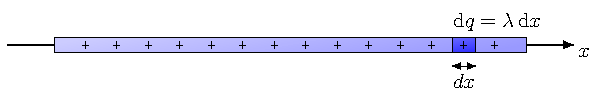
\includegraphics{src/electricfieldline/image1.pdf}
    \label{fig:electricfieldline1}
    \caption{Densità di carica di un filo}
\end{figure}
Se non uniforme
\begin{equation*}
    \lambda = \lambda(x)
\end{equation*}
cioè dipende dalla posizione, e integro in base alla funzione.\\
\textbf{Esempi}
\begin{itemize}
    \item Filo carico uniformemente ($\lambda = \lambda_0$)\\
          Come si trova $\vec{E}$?
          \begin{equation*}
              \vec{E} = \displaystyle \int_{Filo} d \vec{E}
          \end{equation*}
          \begin{equation*}
              \vec{E} = \displaystyle \int_{Filo} \frac{1}{4\pi\varepsilon_0} \cdot \frac{\textcolor{blue}{dq}}{r^2} \cdot \hat{r}
          \end{equation*}
          \begin{equation*}
              \vec{E} = \displaystyle \int_{Filo} k \cdot \frac{\textcolor{blue}{dq}}{r^2} \cdot \hat{r}
          \end{equation*}
          \begin{equation*}
              \overline{\lambda} = \displaystyle \frac{q}{L}
          \end{equation*}
          \begin{equation*}
              \lambda = \lambda_0
          \end{equation*}
          \begin{equation*}
              \lambda_0 = \displaystyle \frac{\textcolor{blue}{dq}}{dx}
          \end{equation*}
          \begin{equation*}
              \textcolor{blue}{dq = \lambda_0 dx}
          \end{equation*}
          \begin{equation*}
              \vec{E} = \displaystyle \int_{Filo} k \cdot \frac{ \textcolor{blue}{\lambda_0 dx}}{r^2} \cdot \hat{r}
          \end{equation*}
          Integrare su tutto il filo significa integrare su $L$.
          \begin{equation*}
              \vec{E} = \displaystyle \int_{0}^{L} k \cdot \frac{ \textcolor{blue}{\lambda_0 dx}}{r^2} \cdot \hat{r}
          \end{equation*}
          \begin{equation*}
              \vec{E} = \displaystyle k \cdot  \frac{1}{r^2} \cdot \hat{r} \cdot \textcolor{blue}{\lambda_0} \int_{0}^{L} \textcolor{blue}{dx}
          \end{equation*}
          \begin{equation*}
              \vec{E} = \displaystyle k \cdot  \frac{1}{r^2} \cdot \hat{r} \cdot \textcolor{blue}{\lambda_0}  \big[ \textcolor{blue}{x}\big]_0^L
          \end{equation*}
          \begin{equation*}
              \vec{E} = \displaystyle k \cdot  \frac{1}{r^2} \cdot \hat{r} \cdot \textcolor{blue}{\lambda_0}  \big[ \textcolor{blue}{L-0} \big]
          \end{equation*}
          \begin{equation*}
              \vec{E} = \displaystyle k \cdot  \frac{1}{r^2} \cdot \hat{r} \cdot \lambda_0 L
          \end{equation*}
          \begin{equation}
              \boxed{\vec{E} = \displaystyle \frac{1}{4\pi\varepsilon_0} \cdot \frac{\lambda_0 L}{r^2} \cdot \hat{r} }
          \end{equation}
          \begin{equation}
              \boxed{\vec{E} = \displaystyle k \cdot \frac{\lambda_0 L}{r^2} \cdot \hat{r} }
          \end{equation}
          \begin{figure}[H]
              \centering
              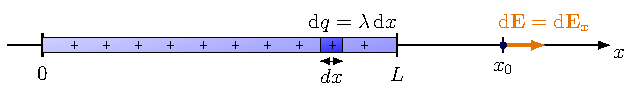
\includegraphics{src/electricfieldline/image2.pdf}
              \label{fig:electricfieldline2}
              \caption{Campo elettrostatico di un filo carico uniformemente}
          \end{figure}


    \item Filo carico non uniformemente ($\lambda(x) = \alpha e^{-x}$)\\
          \begin{equation*}
              \vec{E} = \displaystyle \int_{Filo} d \vec{E}
          \end{equation*}
          \begin{equation*}
              \vec{E} = \displaystyle \int_{Filo} k \cdot \frac{dq}{r^2} \cdot \hat{r}
          \end{equation*}
          \begin{equation*}
              \overline{\lambda} = \displaystyle \frac{q}{L}
          \end{equation*}
          \begin{equation*}
              \lambda = \lambda(x) = \alpha e^{-x}
          \end{equation*}
          \begin{equation*}
              \lambda = \displaystyle \frac{dq}{dx}
          \end{equation*}
          \begin{equation*}
              dq = \lambda dx
          \end{equation*}
          \begin{equation*}
              \vec{E} = \displaystyle \int_{Filo} k \cdot \frac{\lambda dx}{r^2} \cdot \hat{r}
          \end{equation*}
          \begin{equation*}
              \vec{E} = \displaystyle k \cdot \frac{1}{r^2} \cdot \hat{r} \cdot \int_{0}^{L} \lambda\ dx
          \end{equation*}
          \begin{equation*}
              \vec{E} = \displaystyle k \cdot \frac{1}{r^2} \cdot \hat{r} \cdot \int_{0}^{L} \alpha e^{-x}\ dx
          \end{equation*}
          \begin{equation*}
              \vec{E} = \displaystyle k \cdot \frac{1}{r^2} \cdot \hat{r} \cdot \alpha \int_{0}^{L} e^{-x}\ dx
          \end{equation*}
          \begin{equation*}
              \vec{E} = \displaystyle k \cdot \frac{1}{r^2} \cdot \hat{r} \cdot \alpha \bigg[ -e^{-x} \bigg]_0^L
          \end{equation*}
          \begin{equation*}
              \vec{E} = \displaystyle k \cdot \frac{1}{r^2} \cdot \hat{r} \cdot \alpha \bigg[ -e^{-L} - (-e^{-0}) \bigg]
          \end{equation*}
          \begin{equation*}
              \vec{E} = \displaystyle k \cdot \frac{1}{r^2} \cdot \hat{r} \cdot \alpha \bigg[ -e^{-L} + e^{-0} \bigg]
          \end{equation*}
          \begin{equation*}
              \vec{E} = \displaystyle k \cdot \frac{1}{r^2} \cdot \hat{r} \cdot \alpha \left(1 - e^{-L}\right)
          \end{equation*}
\end{itemize}
\subsubsection{Campo elettrostatico di una superficie carica}
Chiamiamo "sigma" la densità superficiale di carica, ovvero la carica per unità di superficie:
\begin{equation*}
    \overline{\sigma} = \displaystyle \frac{q}{S}
\end{equation*}
\begin{equation*}
    \sigma = \displaystyle \frac{dq}{dS}
\end{equation*}
\begin{equation}
    \boxed{dq = \sigma dS}
\end{equation}
\begin{figure}[H]
    \centering
    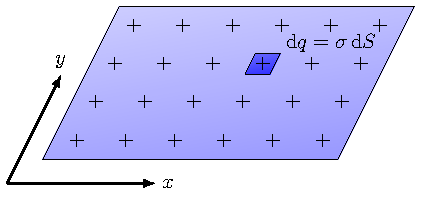
\includegraphics{src/electricfieldplane/image1.pdf}
    \label{fig:electricfieldplane1}
    \caption{Densità di carica di una superficie}
\end{figure}
Se non uniforme
\begin{equation*}
    \sigma = \sigma(x,y) \lor \sigma(r, \theta)
\end{equation*}
cioè dipende dalla posizione, e integro in base alla funzione.\\
\textbf{Esempi(Disco carico)}
\begin{itemize}
    \item Superficie carica uniformemente( $\sigma = \sigma_0$)\\
          \begin{equation*}
              \vec{E} = \displaystyle \int_{Disco} d \vec{E}
          \end{equation*}
          \begin{equation*}
              \vec{E} = \displaystyle \int_{Disco} k \cdot \frac{dq}{r^2} \cdot \hat{r}
          \end{equation*}
          \begin{equation*}
              \overline{\sigma} = \displaystyle \frac{q}{S}
          \end{equation*}
          \begin{equation*}
              \sigma = \sigma_0
          \end{equation*}
          \begin{equation*}
              \sigma_0 = \displaystyle \frac{dq}{dS}
          \end{equation*}
          \begin{equation*}
              dq = \sigma_0 dS
          \end{equation*}
          \begin{equation*}
              \vec{E} = \displaystyle \int_{Disco} k \cdot \frac{\sigma_0 dS}{r^2} \cdot \hat{r}
          \end{equation*}
          \begin{equation*}
              \vec{E} = \displaystyle k \cdot \frac{1}{r^2} \cdot \hat{r} \cdot \int_{Disco} \sigma_0 dS
          \end{equation*}
          \begin{equation*}
              \vec{E} = \displaystyle k \cdot \frac{1}{r^2} \cdot \hat{r} \cdot \sigma_0 \cdot  \int_{Disco} dS
          \end{equation*}
          Integrare su tutto il disco significa integrare su $S$, in questo caso considero le coordinate polari.
          \begin{equation*}
              \vec{E} = \displaystyle k \cdot \frac{1}{r^2} \cdot \hat{r} \cdot \sigma_0 \int_{0}^{2\pi} \int_{0}^{R} x\ dx d\theta
          \end{equation*}
          \begin{equation*}
              \vec{E} = \displaystyle k \cdot \frac{1}{r^2} \cdot \hat{r} \cdot \sigma_0 \int_{0}^{2\pi} \left[\frac{x^2}{2}\right]_0^R d\theta
          \end{equation*}
          \begin{equation*}
              \vec{E} = \displaystyle k \cdot \frac{1}{r^2} \cdot \hat{r} \cdot \sigma_0 \int_{0}^{2\pi} \left[\frac{R^2}{2} - \frac{0^2}{2}\right] d\theta
          \end{equation*}
          \begin{equation*}
              \vec{E} = \displaystyle k \cdot \frac{1}{r^2} \cdot \hat{r} \cdot \sigma_0 \int_{0}^{2\pi} \left[\frac{R^2}{2}\right] d\theta
          \end{equation*}
          \begin{equation*}
              \vec{E} = \displaystyle k \cdot \frac{1}{r^2} \cdot \hat{r} \cdot \sigma_0 \left[\frac{R^2}{2}\right] \int_{0}^{2\pi} d\theta
          \end{equation*}
          \begin{equation*}
              \vec{E} = \displaystyle k \cdot \frac{1}{r^2} \cdot \hat{r} \cdot \sigma_0 \left[\frac{R^2}{2}\right] \big[\theta\big]_0^{2\pi}
          \end{equation*}
          \begin{equation*}
              \vec{E} = \displaystyle k \cdot \frac{1}{r^2} \cdot \hat{r} \cdot \sigma_0 \left[\frac{R^2}{2}\right] \left[2\pi - 0\right]
          \end{equation*}
          \begin{equation*}
              \vec{E} = \displaystyle k \cdot \frac{1}{r^2} \cdot \hat{r} \cdot \sigma_0 \left[\pi R^2\right]
          \end{equation*}
          \begin{figure}[H]
              \centering
              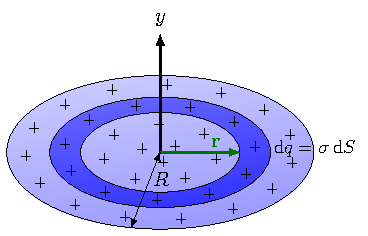
\includegraphics{src/electricfieldplane/image4.pdf}
              \label{fig:electricfieldplane4}
              \caption{Densità di carica di un disco carico}
          \end{figure}
    \item Superficie carica non uniformemente($\sigma(x) = \alpha x$)

\end{itemize}
\subsubsection{Campo elettrostatico di un volume carico}
Chiamiamo "ro" la densità volumetrica di carica, ovvero la carica per unità di volume:
\begin{equation*}
    \overline{\rho} = \displaystyle \frac{q}{V}
\end{equation*}
\begin{equation*}
    \rho = \displaystyle \frac{dq}{dV}
\end{equation*}
\begin{equation}
    \boxed{dq = \rho dV}
\end{equation}
\begin{figure}[H]
    \centering
    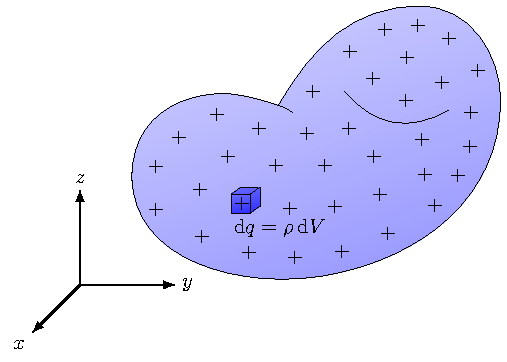
\includegraphics{src/electricfieldvolume/image1.pdf}
    \label{fig:electricfieldvolume1}
    \caption{Densità di carica di un volume}
\end{figure}
Se non uniforme
\begin{equation*}
    \rho = \rho(x,y,z) \lor \rho(r, \phi, \theta) \lor (\rho, \theta, z)
\end{equation*}
cioè dipende dalla posizione, e integro in base alla funzione.\\
\textbf{Esempi(Sfera carica)}
\begin{itemize}
    \item Volume carico uniformemente( $\rho = \rho_0$ )
          \begin{equation*}
              \vec{E} = \displaystyle \int_{Sfera} d \vec{E}
          \end{equation*}
          \begin{equation*}
              \vec{E} = \displaystyle \int_{Sfera} k \cdot \frac{dq}{r^2} \cdot \hat{r}
          \end{equation*}
          \begin{equation*}
              \overline{\rho} = \displaystyle \frac{q}{V}
          \end{equation*}
          \begin{equation*}
              \rho = \rho_0
          \end{equation*}
          \begin{equation*}
              \rho_0 = \displaystyle \frac{dq}{dV}
          \end{equation*}
          \begin{equation*}
              dq = \rho_0 dV
          \end{equation*}
          \begin{equation*}
              \vec{E} = \displaystyle \int_{Sfera} k \cdot \frac{\rho_0 dV}{r^2} \cdot \hat{r}
          \end{equation*}
          \begin{equation*}
              \vec{E} = \displaystyle k \cdot \frac{1}{r^2} \cdot \hat{r} \cdot \int_{Sfera} \rho_0 dV
          \end{equation*}
          \begin{equation*}
              \vec{E} = \displaystyle k \cdot \frac{1}{r^2} \cdot \hat{r} \cdot \rho_0 \cdot  \int_{Sfera} dV
          \end{equation*}
          Integrare su tutto il volume significa integrare su $V$, in questo caso considero le coordinate sferiche, esplicitando bene
          \begin{figure}[H]
              \centering
              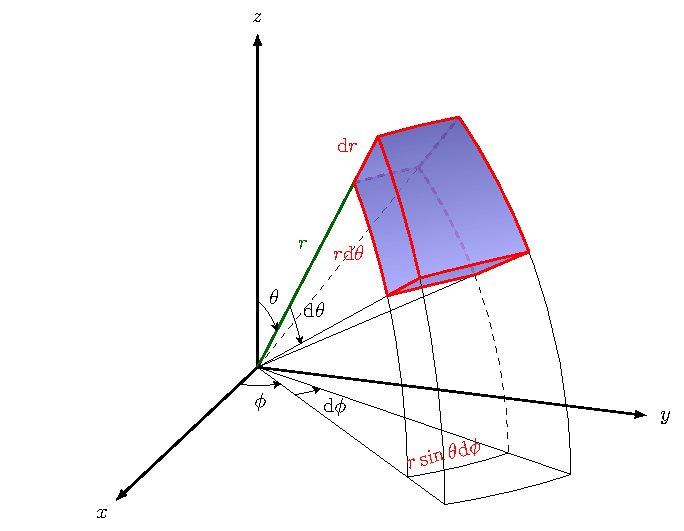
\includegraphics[width=0.5\textwidth]{src/differentialvolumespherical/image1.pdf}
              \label{fig:differentialvolumespherical1}
          \end{figure}
          \begin{equation*}
              dV = r \cdot dr \cdot d\theta \cdot r \cdot \sin(\theta) \cdot d\phi
          \end{equation*}
          \begin{equation*}
              dV = r^2 \sin(\theta) \ dr  d\theta d\phi
          \end{equation*}
          \begin{equation*}
              \vec{E} = \displaystyle k \cdot \frac{1}{r^2} \cdot \hat{r} \cdot \rho_0 \int_{0}^{2\pi} \int_{0}^{\pi} \int_{0}^{R} r^2 \sin(\theta)\ dr d\theta d\phi
          \end{equation*}
          \begin{equation*}
              \vec{E} = \displaystyle k \cdot \frac{1}{r^2} \cdot \hat{r} \cdot \rho_0 \int_{0}^{2\pi} \int_{0}^{\pi} \left[ \frac{r^3}{3} \right]_0^R \sin(\theta)\ d\theta d\phi
          \end{equation*}
          \begin{equation*}
              \vec{E} = \displaystyle k \cdot \frac{1}{r^2} \cdot \hat{r} \cdot \rho_0 \int_{0}^{2\pi} \int_{0}^{\pi} \left[ \frac{R^3}{3} - \frac{0^3}{3} \right] \sin(\theta)\ d\theta d\phi
          \end{equation*}
          \begin{equation*}
              \vec{E} = \displaystyle k \cdot \frac{1}{r^2} \cdot \hat{r} \cdot \rho_0 \int_{0}^{2\pi} \int_{0}^{\pi} \left[ \frac{R^3}{3} \right] \sin(\theta)\ d\theta d\phi
          \end{equation*}
          \begin{equation*}
              \vec{E} = \displaystyle k \cdot \frac{1}{r^2} \cdot \hat{r} \cdot \rho_0 \left[ \frac{R^3}{3} \right] \int_{0}^{2\pi} \int_{0}^{\pi} \sin(\theta)\ d\theta d\phi
          \end{equation*}
          \begin{equation*}
              \vec{E} = \displaystyle k \cdot \frac{1}{r^2} \cdot \hat{r} \cdot \rho_0 \left[ \frac{R^3}{3} \right] \left[ \int_{0}^{2\pi} d\phi \right] \left[ \int_{0}^{\pi} \sin(\theta)\ d\theta \right]
          \end{equation*}
          \begin{equation*}
              \vec{E} = \displaystyle k \cdot \frac{1}{r^2} \cdot \hat{r} \cdot \rho_0 \left[ \frac{R^3}{3} \right] \left[ 2\pi \right] \left[ -\cos(\theta) \right]_0^{\pi}
          \end{equation*}
          \begin{equation*}
              \vec{E} = \displaystyle k \cdot \frac{1}{r^2} \cdot \hat{r} \cdot \rho_0 \left[ \frac{R^3}{3} \right] \left[ 2\pi \right] \left[ -\cos(\pi) + \cos(0) \right]
          \end{equation*}
          \begin{equation*}
              \vec{E} = \displaystyle k \cdot \frac{1}{r^2} \cdot \hat{r} \cdot \rho_0 \left[ \frac{R^3}{3} \right] \left[ 2\pi \right] \left[ -(-1) + 1 \right]
          \end{equation*}
          \begin{equation*}
              \vec{E} = \displaystyle k \cdot \frac{1}{r^2} \cdot \hat{r} \cdot \rho_0 \left[ \frac{R^3}{3} \right] \left[ 2\pi \right] \left[ 2 \right]
          \end{equation*}
          \begin{equation*}
              \vec{E} = \displaystyle k \cdot \frac{1}{r^2} \cdot \hat{r} \cdot \rho_0 \left[ \frac{4}{3}\pi \ R^3 \right]
          \end{equation*}
          \begin{figure}[H]
              \centering
              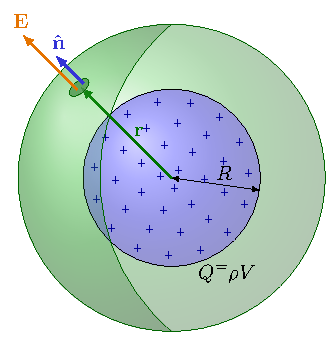
\includegraphics{src/gausslaw/image3.pdf}
              \label{fig:gausslaw3}
              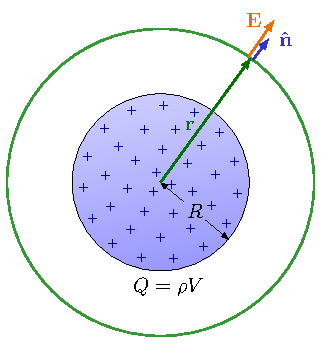
\includegraphics{src/gausslaw/image4.pdf}
              \label{fig:gausslaw4}
          \end{figure}
    \item Volume carico non uniformemente($\rho(x,y,z) = \alpha x^2$)
\end{itemize}

\subsection{Esempi vari}
\subsubsection{Es : Campo elettrostatico di un filo infinito uniformemente carico in un punto P}
\begin{figure}[H]
    \centering
    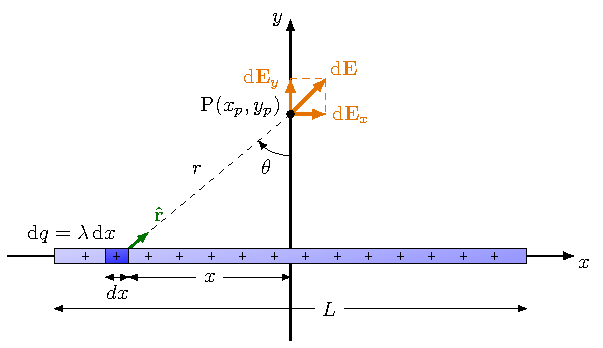
\includegraphics[width=0.45\textwidth]{src/electricfieldline/image4.pdf}
    \label{fig:electricfieldline4}
    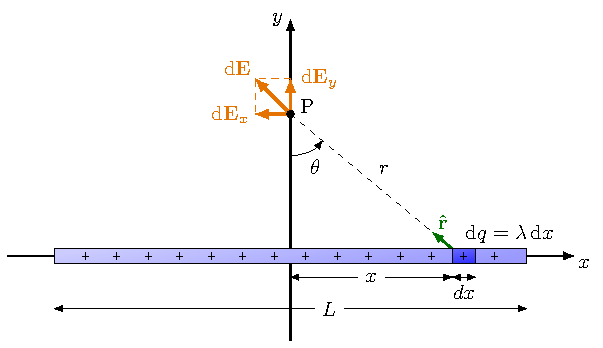
\includegraphics[width=0.45\textwidth]{src/electricfieldline/image3.pdf}
    \label{fig:electricfieldline3}
    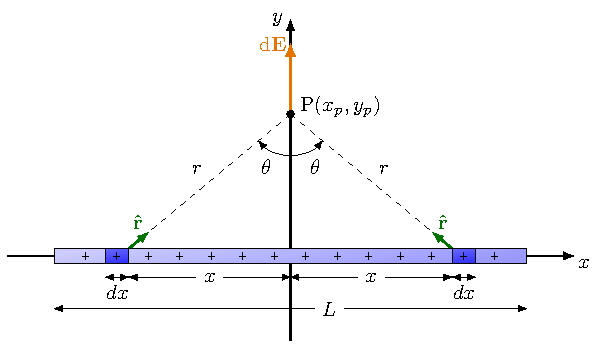
\includegraphics[width=0.6\textwidth]{src/electricfieldline/image5.pdf}
    \label{fig:electricfieldline5}
\end{figure}
Le componenti $d\vec{E}_x$ si annullano,(guarda slides) quindi rimane solo la componente $d\vec{E}_y$.
\begin{equation*}
    d\vec{E} = d \cancel{\vec{E}_x} + d \vec{E}_y
\end{equation*}
\begin{equation*}
    d\vec{E} = d \vec{E}_y
\end{equation*}
\begin{equation*}
    d\vec{E} = k \cdot \frac{dq}{r^2} \cdot \hat{y}
\end{equation*}
\begin{equation*}
    \lambda = \displaystyle \frac{dq}{dx}
\end{equation*}
\begin{equation*}
    dq = \lambda dx
\end{equation*}
\begin{equation*}
    d\vec{E} = k \cdot \frac{\lambda dx}{r^2} \cdot \hat{y}
\end{equation*}
\begin{equation*}
    d E_y = d E \cdot \cos(\theta)
\end{equation*}
\begin{equation*}
    d E_y = k \cdot \frac{\lambda dx}{r^2} \cdot \cos(\theta)
\end{equation*}
\begin{equation*}
    d E_y = k \cdot \frac{\lambda}{r^2} \cdot \cos(\theta) dx
\end{equation*}
\begin{equation*}
    E_y = \displaystyle \int_{Filo} k \cdot \frac{\lambda}{r^2} \cdot \cos(\theta) dx
\end{equation*}
Questo è un problema a un grado di libertà: le tre variabili $\theta, x, r$ sono correlate tra loro.\\
\begin{equation*}
    \begin{cases}
        y_p = r \cdot \cos(\theta) \\
        x = y_p \cdot \tan(\theta) \\
    \end{cases}
\end{equation*}
\begin{equation*}
    \begin{cases}
        y_p = r \cdot \cos(\theta)                            \\
        dx = \displaystyle \frac{dy_p}{\cos^2(\theta)}d\theta \\
    \end{cases}
\end{equation*}
\begin{equation*}
    \begin{cases}
        r = \displaystyle \frac{y_p}{\cos(\theta)}             \\
        dx = \displaystyle \frac{dy_p}{\cos^2(\theta)} d\theta \\
    \end{cases}
\end{equation*}
\begin{equation*}
    \begin{cases}
        \textcolor{blue}{r^{-2} = \displaystyle \frac{\cos^2(\theta)}{y_p^2}}       \\
        \textcolor{violet}{dx = \displaystyle \frac{dy_p}{\cos^2(\theta)} d\theta } \\
    \end{cases}
\end{equation*}
\begin{equation*}
    E_y = \displaystyle \int_{Filo} k \cdot \frac{\lambda}{r^2} \cdot \cos(\theta) \cdot dx
\end{equation*}
\begin{equation*}
    E_y = \displaystyle \int_{Filo} k \cdot \frac{\lambda\textcolor{blue}{\cos^2(\theta)}}{\textcolor{blue}{y_p^2}} \cdot \cos(\theta) \cdot \textcolor{violet}{\frac{dy_p}{\cos^2(\theta)} d\theta }
\end{equation*}
\begin{equation*}
    E_y = \displaystyle \int_{Filo} k \cdot \frac{\lambda}{y_p} \cdot \cos(\theta) d\theta
\end{equation*}
\begin{equation*}
    E_y = \displaystyle k \cdot \lambda \cdot \frac{1}{y_p} \int_{Filo} \cos(\theta) d\theta
\end{equation*}
Integrare su tutto il filo significa integrare sull'angolo $\theta$.
\begin{equation*}
    E_y = \displaystyle k \cdot \lambda \cdot \frac{1}{y_p} \int_{-\frac{\pi}{2}}^{\frac{\pi}{2}} \cos(\theta) d\theta
\end{equation*}
\begin{equation*}
    E_y = \displaystyle k \cdot \lambda \cdot \frac{1}{y_p} \Big[ \sin(\theta) \Big]_{-\frac{\pi}{2}}^{\frac{\pi}{2}}
\end{equation*}
\begin{equation*}
    E_y = \displaystyle k \cdot \lambda \cdot \frac{1}{y_p} \left[ \sin\left(\frac{\pi}{2}\right) - \sin\left(-\frac{\pi}{2}\right) \right]
\end{equation*}
\begin{equation*}
    E_y = \displaystyle k \cdot \lambda \cdot \frac{1}{y_p} \left[ 1 - (-1) \right]
\end{equation*}
\begin{equation*}
    E_y = \displaystyle k \cdot \lambda \cdot \frac{1}{y_p} \left[ 2 \right]
\end{equation*}
\begin{equation*}
    E_y = \displaystyle k \cdot \lambda \cdot \frac{2}{y_p}
\end{equation*}
\begin{equation*}
    E_y = \displaystyle \frac{\lambda }{2 \pi \varepsilon_0} \cdot \frac{1}{y_p}
\end{equation*}
\begin{equation}
    \boxed{\vec{E} = \displaystyle \frac{\lambda }{2 \pi \varepsilon_0} \cdot \frac{1}{y_p} \hat{y}}
\end{equation}

\subsubsection{Es : Campo elettrostatico di un piano infinito e densità superficiale di carica uniforme}
\begin{figure}[H]
    \centering
    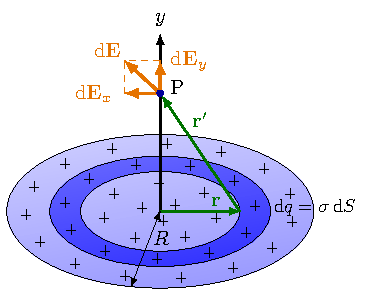
\includegraphics{src/electricfieldplane/image3.pdf}
    \label{fig:electricfieldplane3}
\end{figure}
Il ragionamento è simile a quello del filo.
\begin{equation}
    \boxed{\vec{E} = \displaystyle \frac{\sigma}{2\varepsilon_0} \hat{n}}
\end{equation}
\textbf{Osservazioni}
\begin{itemize}
    \item Il campo elettrostatico di un piano infinito \textbf{non dipende dalla distanza dal piano}.
\end{itemize}
What's $\hat{n}$?\\
$\hat{n}$ è il versore normale alla superficie, ovvero il versore perpendicolare alla superficie, si considera uscente.\\
\subsection{Campo elettrostatico tra due lastre cariche}
Il campo elettrostatico tra due lastre cariche è uniforme e diretto da quella positiva a quella negativa.
\begin{equation*}
    \vec{E} = \vec{E}_+ + \vec{E}_-
\end{equation*}
\begin{equation*}
    \vec{E} = \displaystyle \frac{\sigma}{2\varepsilon_0} \hat{n} + \displaystyle \frac{\sigma}{2\varepsilon_0} \hat{n}
\end{equation*}
\begin{equation}
    \boxed{\vec{E} = \displaystyle \frac{\sigma}{\varepsilon_0} \hat{n}}
\end{equation}
Il campo elettrostatico all'esterno delle lastre è nullo.
\begin{figure}[H]
    \centering
    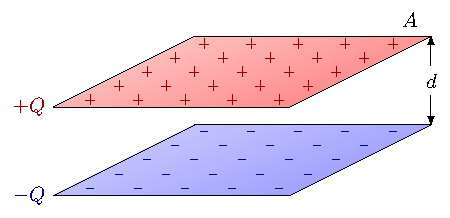
\includegraphics{src/capacitors/image1.pdf}
    \label{fig:capacitors1}
    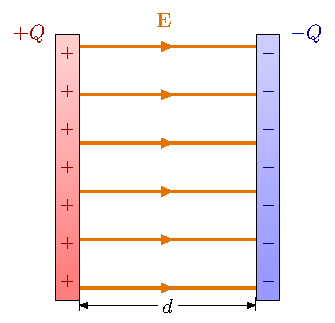
\includegraphics{src/capacitors/image2.pdf}
    \label{fig:capacitors2}
\end{figure}
\subsubsection{Es : Moto di una particella carica in un campo elettrostatico}
Viene richiesto di calcolare la velocità con cui un elettrone esce dal buco.\\
Molto easy, si calcola il campo elettrostatico in un punto P, e si calcola la forza di Coulomb, e si calcola l'accelerazione, e si calcola la velocità.\\
\subsection{Formule utili}
\textbf{Costanti}
\begin{equation}
    k = \displaystyle \frac{1}{4\pi\varepsilon_0} = 8.99 \cdot 10^9 \ \frac{N \cdot m^2}{C^2}
\end{equation}
\begin{equation}
    \varepsilon_0 = 8.85 \cdot 10^{-12} \ \frac{C^2}{N \cdot m^2}
\end{equation}
\begin{equation}
    e = 1.6 \cdot 10^{-19} \ C
\end{equation}
\begin{equation}
    m_e = 9.11 \cdot 10^{-31} \ kg
\end{equation}
\begin{equation}
    m_p = 1.67 \cdot 10^{-27} \ kg
\end{equation}
\textbf{Forza di Coulomb}
\begin{equation}
    \boxed{\vec{F} = \displaystyle \frac{1}{4\pi\varepsilon_0} \cdot \frac{q_1 \cdot q_2}{r^2} \cdot \hat{r}}
\end{equation}
\begin{equation}
    \boxed{\vec{F} = \displaystyle k \cdot \frac{q_1 \cdot q_2}{r^2} \cdot \hat{r}}
\end{equation}
\begin{equation}
    \boxed{\vec{F} = q \cdot \vec{E}}
\end{equation}
\textbf{Campo elettrostatico}
\begin{equation}
    \boxed{\vec{E} = \displaystyle \frac{1}{4\pi\varepsilon_0} \cdot \frac{q}{r^2} \cdot \hat{r}}
\end{equation}
\begin{equation}
    \boxed{\vec{E} = \displaystyle k \cdot \frac{q}{r^2} \cdot \hat{r}}
\end{equation}
\begin{equation}
    \boxed{\vec{E} = \int_{Corpo} d \vec{E}}
\end{equation}
\begin{equation}
    \boxed{\vec{E} = \int_{Corpo} \displaystyle k \cdot \frac{dq}{r^2} \cdot \hat{r}}
\end{equation}
\textbf{Densità di carica}
\begin{equation}
    \boxed{dq = \lambda dx}
\end{equation}
\begin{equation}
    \boxed{dq = \sigma dS}
\end{equation}
\begin{equation}
    \boxed{dq = \rho dV}
\end{equation}
\textbf{Campo elettrostatico di situazioni note}\\
\noindent
Filo carico uniformemente
\begin{equation}
    \boxed{\vec{E} = \displaystyle \frac{\lambda }{2 \pi \varepsilon_0} \cdot \frac{1}{y_p} \hat{y}}
\end{equation}
Lastra carica uniformemente
\begin{equation}
    \boxed{\vec{E} = \displaystyle \frac{\sigma}{2\varepsilon_0} \hat{n}}
\end{equation}
Due lastre cariche uniformemente
\begin{equation}
    \boxed{\vec{E} = \displaystyle \frac{\sigma}{\varepsilon_0} \hat{n}}
\end{equation}
\newpage
\section{Legge di Gauss}
\subsection{Flusso}
\subsubsection{Flusso di campo vettoriale}
\begin{small}
    \paragraph{Flusso di un campo vettoriale}
    La nozione di \textbf{flusso} nasce in fluidodinamica ed è intesa come \textbf{portata di un fluido attraverso una superficie orientata}.\\
    In parole semplici, è la quantità di fluido che attraversa una superficie in un certo periodo di tempo.\\
    \begin{figure}[H]
        \centering
        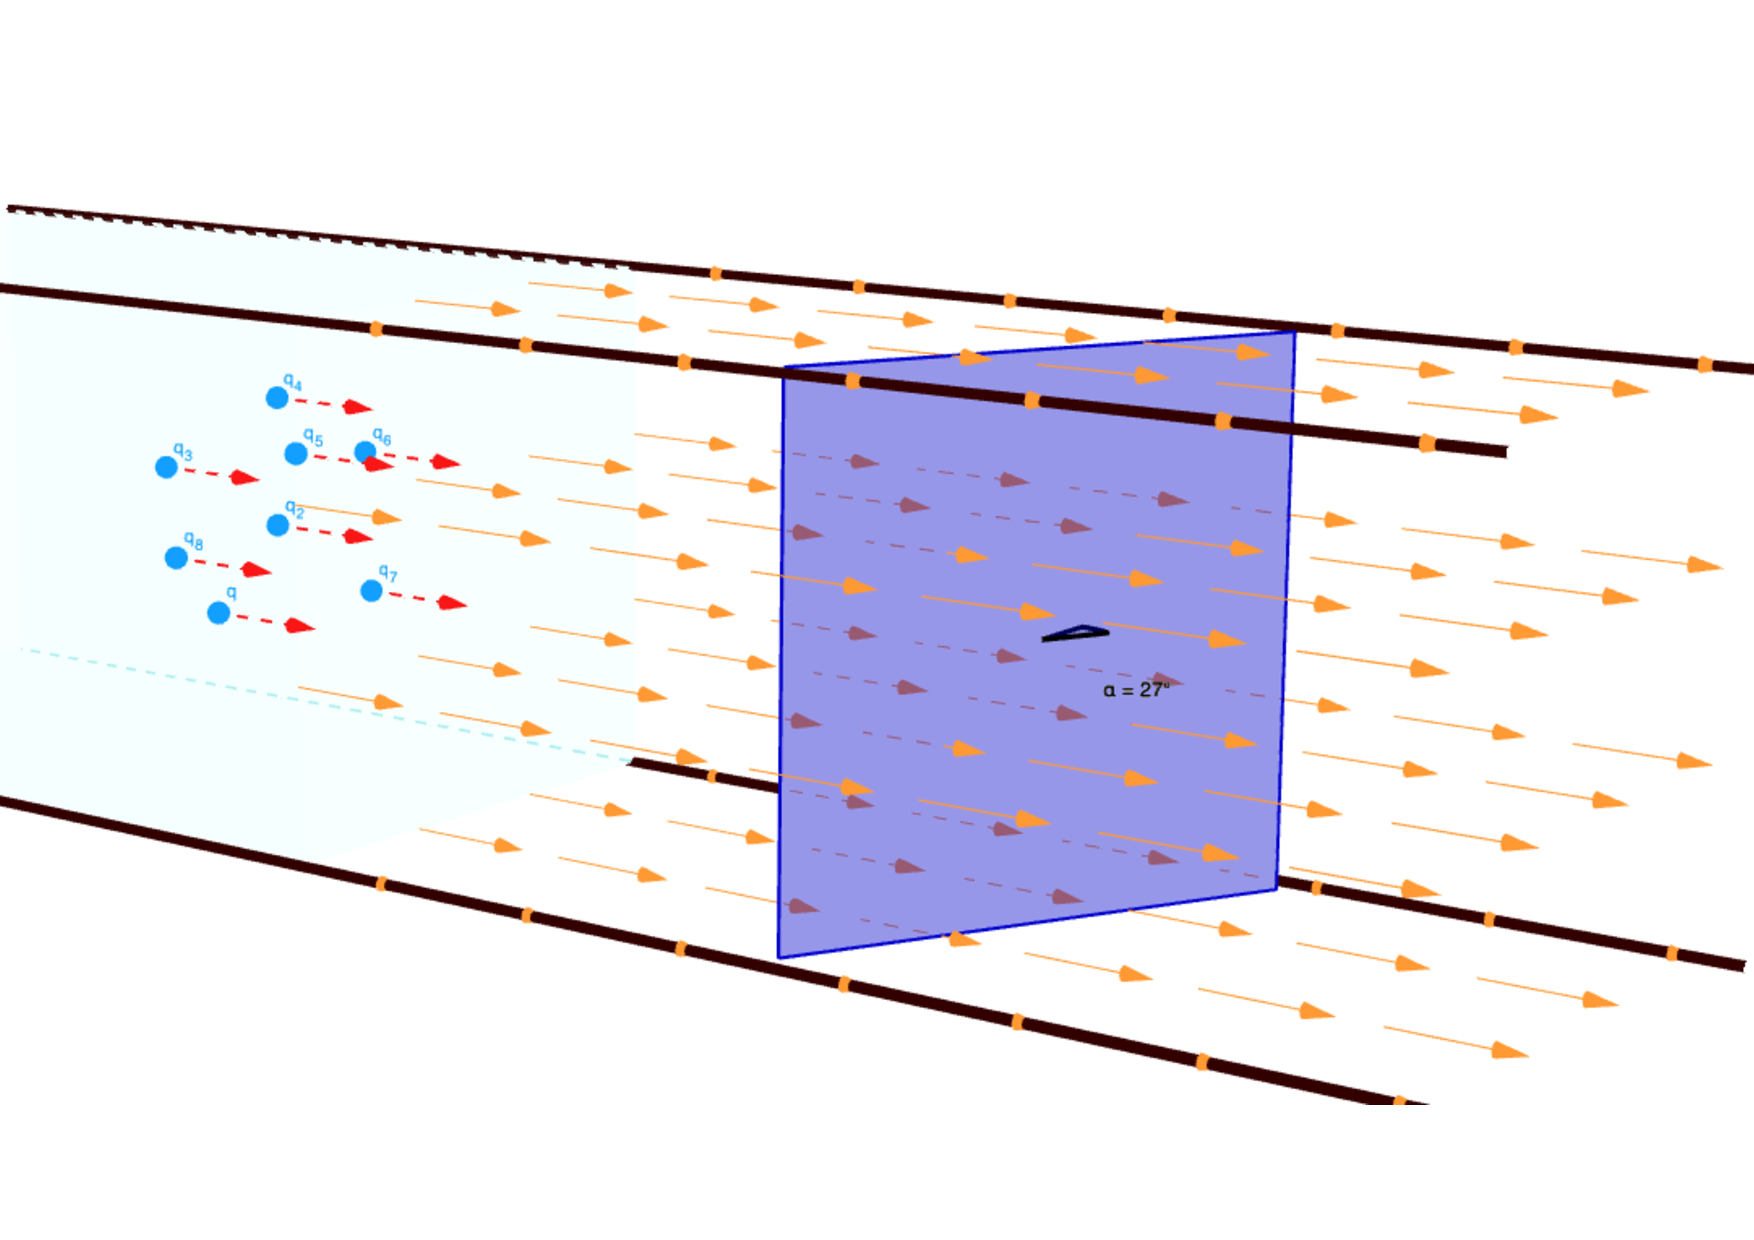
\includegraphics[width=0.5\textwidth]{src/electricflux/image1.pdf}
        \label{fig:electricflux1}
    \end{figure}
    Il \textbf{flusso elementare} $d \Phi_{\vec{F}}$ di un campo vettoriale $\vec{F}$( nota intendo un qualsiasi campo vettoriale e gli sto assegnando il simbolo $\vec{F}$) attraverso una \textbf{porzione elementare di superficie} $d\vec{S}$ è definito come il \textbf{prodotto scalare} tra il campo vettoriale e il vettore normale alla superficie.\\
    \begin{equation}
        \boxed{d\Phi = \vec{F} \cdot d\vec{S} = \vec{F} \cdot dS \cdot \hat{n}}
    \end{equation}
    \begin{figure}[H]
        \centering
        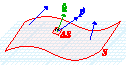
\includegraphics[width=0.35\textwidth]{src/electricflux/image2.pdf}
        \label{fig:electricflux2}
    \end{figure}
\end{small}
Il \textbf{flusso totale} $\Phi_{\vec{F}}$ di un campo vettoriale $\vec{F}$ attraverso una superficie $S$ è definito come la somma dei flussi elementari su tutta la superficie.\\
Esso è uno \textbf{scalare}.
\begin{equation*}
    \Phi_{\vec{F}} \displaystyle = \int_{S} \vec{F} \cdot dS \cdot \hat{n}
\end{equation*}
\begin{equation*}
    \Phi_{\vec{F}} \displaystyle = \int_{S} \vec{F} \cdot d\vec{S}
\end{equation*}
\begin{equation*}
    \Phi_{\vec{F}} \displaystyle = \int_{S} d\Phi_{\vec{F}}
\end{equation*}
\begin{equation}
    \boxed{\Phi_{\vec{F}} \displaystyle = \int_{S} d\Phi_{\vec{F}}}
\end{equation}
\begin{figure}[H]
    \centering
    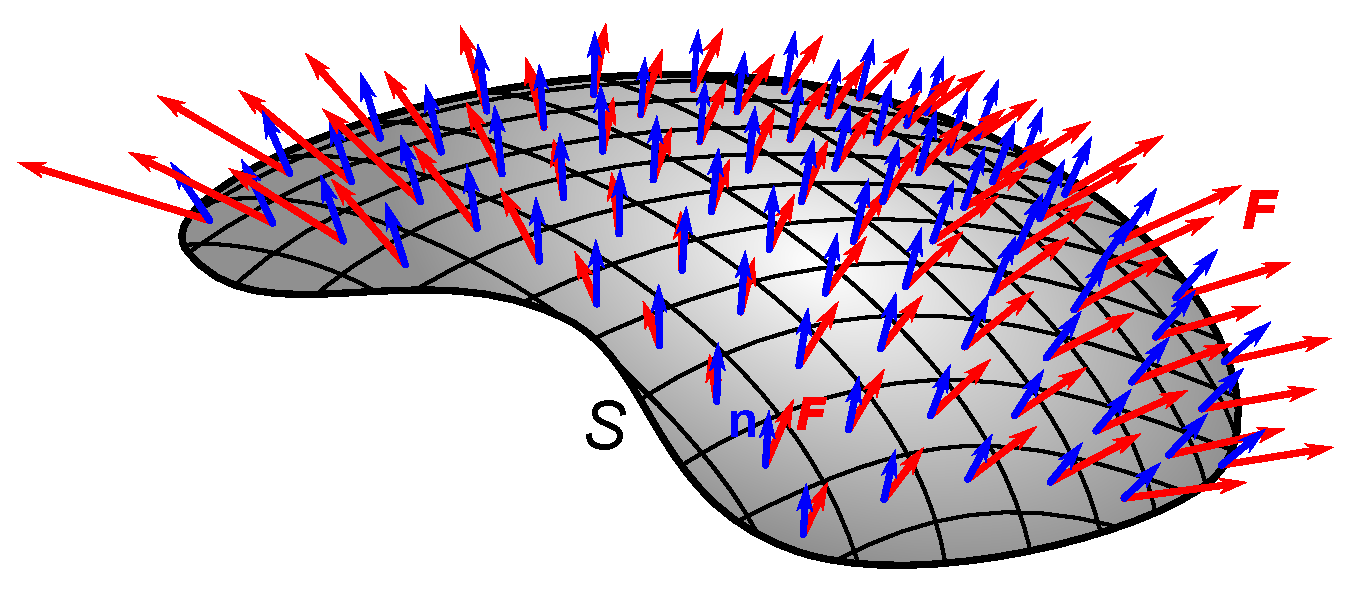
\includegraphics[width=0.35\textwidth]{src/electricflux/image3.pdf}
    \label{fig:electricflux3}
\end{figure}

\subsubsection{Flusso di un campo elettrostatico}
Il \textbf{flusso} del campo elettrostatico \textbf{è proporzionale} al numero di linee di campo che attraversano la superficie di area $S$.\\
\begin{equation}
    \boxed{\Phi_{\vec{E}} = \displaystyle \int_{S} \vec{E} \cdot d\vec{S}}
    \label{eq:gausslaw1}
\end{equation}
\textbf{Flusso di un campo elettrostatico uniforme attraverso una superficie piana}
\begin{equation}
    \boxed{\Phi_{\vec{E}} = \vec{E} \cdot \vec{S}}
\end{equation}
\begin{figure}[H]
    \centering
    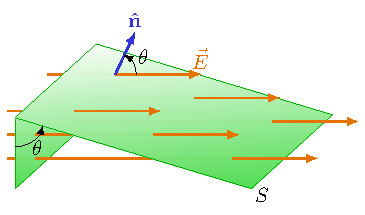
\includegraphics[width=0.35\textwidth]{src/electricflux/image4.pdf}
    \label{fig:electricflux4}
\end{figure}
\begin{itemize}
    \item $\theta = 0 \quad \vec{E} \parallel \hat{n}$
          \begin{equation*}
              \Phi_{\vec{E}} = E \cdot S \cdot \cos(0)
          \end{equation*}
          \begin{equation*}
              \Phi_{\vec{E}} = E \cdot S \cdot 1
          \end{equation*}
          \begin{equation*}
              \Phi_{\vec{E}} = E \cdot S
          \end{equation*}
    \item $\theta = 90 \quad \vec{E} \perp \hat{n}$
          \begin{equation*}
              \Phi_{\vec{E}} = E \cdot S \cdot \cos(90)
          \end{equation*}
          \begin{equation*}
              \Phi_{\vec{E}} = E \cdot S \cdot 0
          \end{equation*}
    \item $\theta = \theta_0$
          \begin{equation*}
              \Phi_{\vec{E}} = E \cdot S \cdot \cos(\theta_0)
          \end{equation*}
\end{itemize}
\textbf{Flusso di un campo elettrostatico uniforme che attraversa una superficie chiusa}\\
Nel caso di una superficie chiusa attraversata da un campo elettrostatico il suo flusso è nullo.\\
\begin{equation}
    \boxed{\Phi_{\vec{E}} = 0}
    \label{eq:gausslaw3}
\end{equation}
Nota:
\begin{itemize}
    \item $\hat{n}$ è sempre uscente, di conseguenza anche $d\vec{S}$.
    \item Il campo in questo esempio è generato da una sorgente esterna alla superficie.
\end{itemize}
\begin{figure}[H]
    \centering
    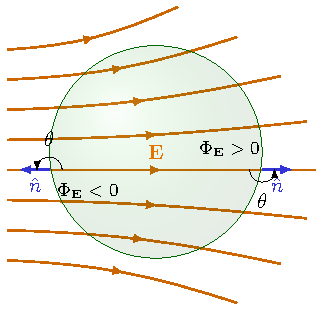
\includegraphics[width=0.35\textwidth]{src/gausslaw/image2.pdf}
    \label{fig:gausslaw2}
\end{figure}
\subsection{Legge di Gauss}
\subsubsection{Legge di Gauss}
Il \textbf{flusso} del campo elettrico attraverso una qualsiasi \textbf{superficie chiusa} dipende solo dalla somma algebrica delle cariche contenute all'interno della superficie.\\
\begin{equation}
    \boxed{\Phi_{\vec{E}} = \displaystyle \frac{1}{\varepsilon_0} \sum_{i=1}^{n} q_{i}^{int}}
    \label{eq:gausslaw2}
\end{equation}
\textbf{Nota:}
\begin{itemize}
    \item \textcolor{red}{IMPORTANTE} : Nonostante la legge di Gauss \ref{eq:gausslaw2}, ciò non significa che il campo $\vec{E}$ che troviamo nella \ref{eq:gausslaw1} è generato solo dalle cariche interne alla superficie.
    \item La superficie chiusa è chiamata \textbf{superficie gaussiana}, è un ente geometrico non deve essere per forza fisico.
\end{itemize}
\begin{figure}[H]
    \centering
    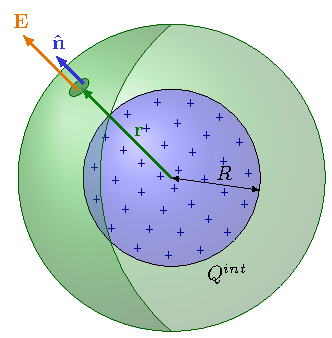
\includegraphics[width=0.35\textwidth]{src/gausslaw/image6.pdf}
    \label{fig:gausslaw6}
\end{figure}
\subsubsection{Legge di Gauss e distribuzione di carica continua}
\begin{equation}
    \boxed{\Phi_{\vec{E}} = \displaystyle \frac{1}{\varepsilon_0} \cdot \int_{Corpo} d\ q^{int}}
\end{equation}
\begin{equation*}
    \begin{cases}
        \Phi_{\vec{E}} = \displaystyle \frac{1}{\varepsilon_0} \cdot \int_{Filo} \lambda dl \\
        \\
        \Phi_{\vec{E}} = \displaystyle \frac{1}{\varepsilon_0} \cdot \int_{Piano} \sigma dS \\
        \\
        \Phi_{\vec{E}} = \displaystyle \frac{1}{\varepsilon_0} \cdot \int_{Sfera} \rho dV   \\
    \end{cases}
\end{equation*}
\newpage
\subsection{Esempi vari}
Di seguito alcune applicazioni della legge di Gauss.
\subsubsection{Es : Campo elettrostatico interno ed esterno ad un guscio carico sottile (2D)}\label{sec:esempiogausslaw}
\begin{figure}[H]
    \centering
    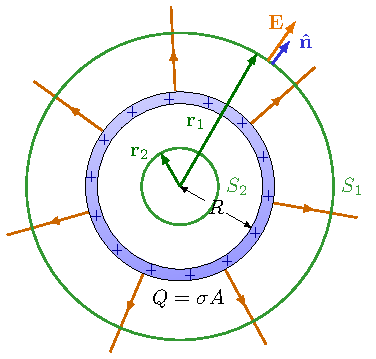
\includegraphics[width=0.35\textwidth]{src/gausslaw/image7.pdf}
    \label{fig:gausslaw7}
\end{figure}
\begin{itemize}
    \item All'\textbf{esterno} del guscio prendo una superficie gaussiana sferica $S_1$.\\
          \begin{multicols}{2}
              \noindent
              Dalla definizione di flusso \ref{eq:gausslaw1}
              \begin{equation*}
                  \Phi_{\vec{E}} = \displaystyle \int_{S} \vec{E} \cdot d\vec{S}
              \end{equation*}
              \columnbreak
              \noindent

              Dalla legge di Gauss \ref{eq:gausslaw2}
              \begin{equation*}
                  \Phi_{\vec{E}} = \displaystyle \frac{Q^{int}}{\varepsilon_0}
              \end{equation*}
          \end{multicols}
          \begin{equation*}
              \Phi_{\vec{E}} = \displaystyle \int_{S_1} \vec{E} \cdot d\vec{S}_1
          \end{equation*}
          \begin{equation*}
              \displaystyle \frac{Q}{\varepsilon_0} = \displaystyle \int_{S_1} \vec{E} \cdot d\vec{S}_1
          \end{equation*}
          \begin{equation*}
              \displaystyle \frac{Q}{\varepsilon_0} = \vec{E} \cdot \displaystyle \int_{S_1} d\vec{S}_1
          \end{equation*}
          \begin{equation*}
              \displaystyle \frac{Q}{\varepsilon_0} = \vec{E} \cdot \vec{S}_1
          \end{equation*}
          \begin{equation*}
              \vec{E} = \displaystyle \frac{Q}{\varepsilon_0} \cdot \frac{1}{S_1}
          \end{equation*}
          \begin{equation}
              \boxed{\vec{E} = \displaystyle \frac{Q}{4\pi \varepsilon_0 r_{1}^2}}
          \end{equation}
    \item All'\textbf{interno} del guscio prendo una superficie gaussiana sferica $S_2$.\\
          \begin{multicols}{2}
              \noindent
              Dalla definizione di flusso \ref{eq:gausslaw1}
              \begin{equation*}
                  \Phi_{\vec{E}} = \displaystyle \int_{S} \vec{E} \cdot d\vec{S}
              \end{equation*}
              \columnbreak
              \noindent

              Dalla legge di Gauss \ref{eq:gausslaw2}
              \begin{equation*}
                  \Phi_{\vec{E}} = \displaystyle \frac{Q^{int}}{\varepsilon_0}
              \end{equation*}
          \end{multicols}
          \begin{equation*}
              \Phi_{\vec{E}} = \displaystyle \frac{Q^{int}}{\varepsilon_0}
          \end{equation*}
          \begin{equation*}
              \Phi_{\vec{E}} = \displaystyle \frac{0}{\varepsilon_0}
          \end{equation*}
          \begin{equation*}
              \Phi_{\vec{E}} = 0
          \end{equation*}
          \begin{equation*}
              \Phi_{\vec{E}} = \displaystyle \int_{S_2} \vec{E} \cdot d\vec{S}_2
          \end{equation*}
          \begin{equation*}
              \displaystyle 0 = \displaystyle \int_{S_2} \vec{E} \cdot d\vec{S}_2
          \end{equation*}
          \begin{equation*}
              \displaystyle 0 = \vec{E} \cdot \displaystyle \int_{S_2} d\vec{S}_2
          \end{equation*}
          \begin{equation*}
              \displaystyle 0 = \vec{E} \cdot \vec{S}_2
          \end{equation*}
          \begin{equation}
              \boxed{\vec{E} = 0}
              \label{eq:gausslaw4}
          \end{equation}
\end{itemize}
Ricapitolando:
\begin{equation}
    \boxed{\vec{E} =
        \begin{cases}
            \displaystyle \frac{Q}{4\pi \varepsilon_0 r_{1}^2} & \text{se esterno } r_1 > R \\
            \\
            0                                                  & \text{se interno } r_2 < R \\
        \end{cases}
    }
\end{equation}
\begin{figure}[H]
    \centering
    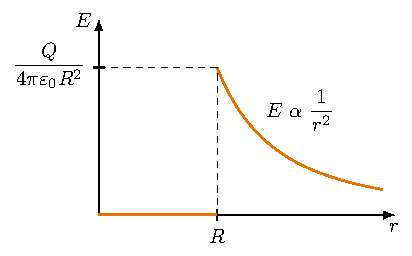
\includegraphics[width=0.35\textwidth]{src/electricfieldplot/image1.pdf}
    \label{fig:electricfieldplot1}
\end{figure}

\subsubsection{Es : Campo elettrostatico interno ed esterno ad una sfera uniformemente carico (3D)}
\textbf{Dati}
\begin{itemize}
    \item Raggio sfera $R$
    \item Densità volumetrica di carica $\rho$
    \item Raggio sfera gaussiana esterna $r_1$
    \item Raggio sfera gaussiana interna $r_2$
\end{itemize}
\begin{figure}[H]
    \centering
    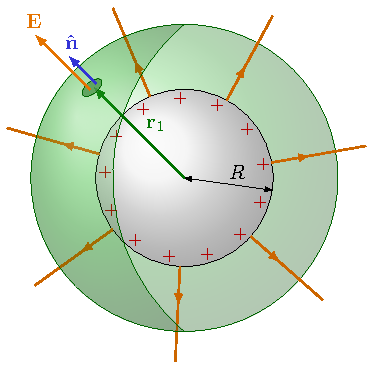
\includegraphics[width=0.35\textwidth]{src/gausslaw/image9.pdf}
    \label{fig:gausslaw9}
    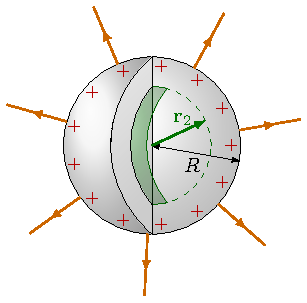
\includegraphics[width=0.35\textwidth]{src/gausslaw/image10.pdf}
    \label{fig:gausslaw10}
\end{figure}
\begin{itemize}
    \item All'\textbf{esterno} della sfera prendo una superficie gaussiana sferica $S_1$.\\
          \begin{multicols}{2}
              \noindent
              Dalla definizione di flusso \ref{eq:gausslaw1}
              \begin{equation*}
                  \Phi_{\vec{E}} = \displaystyle \int_{S} \vec{E} \cdot d\vec{S}
              \end{equation*}
              \columnbreak
              \noindent

              Dalla legge di Gauss \ref{eq:gausslaw2}
              \begin{equation*}
                  \Phi_{\vec{E}} = \displaystyle \frac{Q^{int}}{\varepsilon_0}
              \end{equation*}
          \end{multicols}
          \begin{equation*}
              \Phi_{\vec{E}} = \displaystyle \int_{S_1} \vec{E} \cdot d\vec{S}_1
          \end{equation*}
          \begin{equation*}
              \displaystyle \frac{Q}{\varepsilon_0} = \displaystyle \int_{S_1} \vec{E} \cdot d\vec{S}_1
          \end{equation*}
          \begin{equation*}
              \displaystyle \frac{Q}{\varepsilon_0} = \vec{E} \cdot \displaystyle \int_{S_1} d\vec{S}_1
          \end{equation*}
          \begin{equation*}
              \displaystyle \frac{Q}{\varepsilon_0} = \vec{E} \cdot \vec{S}_1
          \end{equation*}
          \begin{equation*}
              \vec{E} = \displaystyle \frac{Q}{\varepsilon_0} \cdot \frac{1}{S_1}
          \end{equation*}
          \begin{equation}
              \vec{E} = \displaystyle \frac{Q}{4\pi \varepsilon_0} \cdot \frac{1}{r_{1}^{2}}
          \end{equation}
          \begin{equation}
              \boxed{\vec{E} = \displaystyle \frac{Q}{4\pi \varepsilon_0 r_{1}^2}}
          \end{equation}
          dove
          \begin{equation*}
              Q = \rho \cdot V_{sfera}
          \end{equation*}
          \begin{equation*}
              Q = \rho \cdot \frac{4}{3} \pi R^3
          \end{equation*}
    \item All'\textbf{interno} della sfera prendo una superficie gaussiana sferica $S_2$.\\
          \begin{multicols}{2}
              \noindent
              Dalla definizione di flusso \ref{eq:gausslaw1}
              \begin{equation*}
                  \Phi_{\vec{E}} = \displaystyle \int_{S_2} \vec{E} \cdot d\vec{S}_2
              \end{equation*}
              \begin{equation*}
                  \Phi_{\vec{E}} = \displaystyle  \vec{E} \cdot \vec{S}_2
              \end{equation*}
              \begin{equation*}
                  \underline{\Phi_{\vec{E}} = \vec{E} \cdot 4\pi r_{2}^2}
              \end{equation*}
              \columnbreak
              \noindent

              Dalla legge di Gauss \ref{eq:gausslaw2} sappiamo che
              \begin{equation*}
                  \Phi_{\vec{E}} = \displaystyle \frac{Q^{int}}{\varepsilon_0}
              \end{equation*}
              Importante notare che $Q^{int}$ è la carica contenuta all'interno della superficie gaussiana $S_2$ \textbf{NON} la carica della sfera .\\
              \begin{equation*}
                  Q^{int} = \rho \cdot V_{S_2}
              \end{equation*}
              \begin{equation*}
                  Q^{int} = \rho \cdot \frac{4}{3} \pi r_{2}^3
              \end{equation*}
              Tornando al flusso
              \begin{equation*}
                  \Phi_{\vec{E}} = \displaystyle \frac{\rho \cdot \frac{4}{3} \pi r_{2}^3}{\varepsilon_0}
              \end{equation*}
              \begin{equation*}
                  \Phi_{\vec{E}} = \displaystyle \frac{4}{3} \cdot \frac{1}{\varepsilon_0} \rho \cdot  \pi r_{2}^3
              \end{equation*}
              Ma $\rho$
              \begin{equation*}
                  \rho = \displaystyle \frac{Q}{V_{sfera}}
              \end{equation*}
              \begin{equation*}
                  \rho = \displaystyle \frac{Q}{\frac{4}{3} \pi R^3}
              \end{equation*}
              \begin{equation*}
                  \rho = \displaystyle \frac{3Q}{4 \pi R^3}
              \end{equation*}
              Tornando al flusso
              \begin{equation*}
                  \Phi_{\vec{E}} = \displaystyle \frac{4}{3} \cdot \frac{1}{\varepsilon_0} \cdot \frac{3Q}{4 \pi R^3} \cdot  \pi r_{2}^3
              \end{equation*}
              \begin{equation*}
                  \underline{\Phi_{\vec{E}} = \displaystyle \frac{Q}{\varepsilon_0} \cdot \frac{r_{2}^3}{R^3}}
              \end{equation*}
          \end{multicols}
          Uguagliamo le due espressioni di $\Phi_{\vec{E}}$
          \begin{equation*}
              \displaystyle \vec{E} \cdot 4\pi r_{2}^2 = \frac{Q}{\varepsilon_0} \cdot \frac{r_{2}^3}{R^3}
          \end{equation*}
          \begin{equation*}
              \displaystyle \vec{E} \cdot 4\pi = \frac{Q}{\varepsilon_0} \cdot \frac{r_{2}}{R^3}
          \end{equation*}
          \begin{equation*}
              \vec{E} = \displaystyle \frac{Q}{4\pi \varepsilon_0} \cdot \frac{r_{2}}{R^3} \hat{r}
          \end{equation*}
          \begin{equation}
              \boxed{\vec{E} = \displaystyle \frac{Q}{4\pi \varepsilon_0 R^3} \cdot r_{2} \hat{r}}
          \end{equation}
\end{itemize}
Ricapitolando
\begin{equation}
    \boxed{\vec{E} =
        \begin{cases}
            \displaystyle \frac{Q}{4\pi \varepsilon_0 r^2}         & \text{se esterno } r > R \\
            \\
            \displaystyle \frac{Q}{4\pi \varepsilon_0 R^3} \cdot r & \text{se interno } r < R \\
        \end{cases}
    }
\end{equation}
\begin{figure}[H]
    \centering
    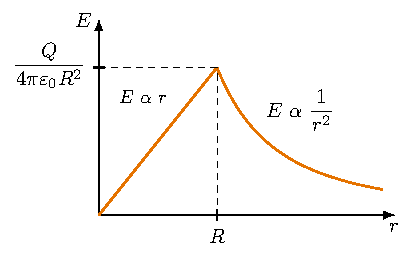
\includegraphics[width=0.35\textwidth]{src/electricfieldplot/image2.pdf}\\
    \label{fig:electricfieldplot2}
\end{figure}

\subsection{Teorema di Coulomb}

Il campo elettrico sulla superficie di un \textbf{conduttore} è sempre \textbf{perpendicolare alla superficie} del conduttore a prescindere dalla forma.\\
\begin{figure}[H]
    \centering
    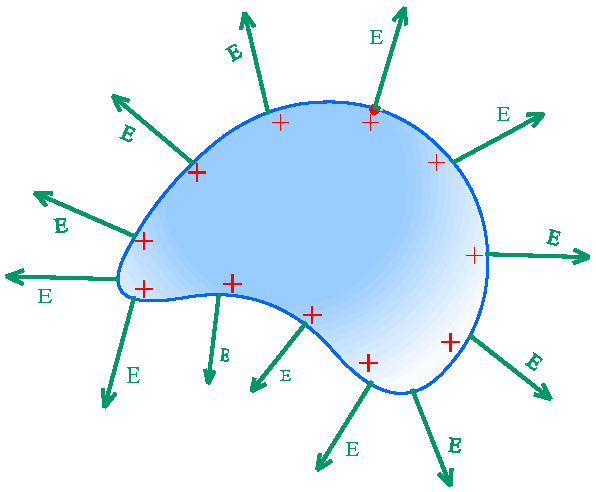
\includegraphics[width=0.35\textwidth]{src/coulombtheorem/image2.pdf}
    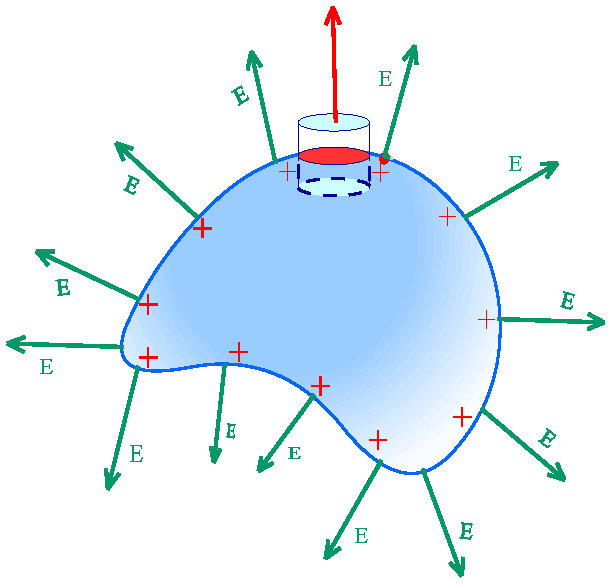
\includegraphics[width=0.35\textwidth]{src/coulombtheorem/image1.pdf}
\end{figure}
\noindent
\textbf{Dimostrazione}\\
Considero un cilindro gaussiano che racchiude un \(dS = S_{Base\ cilindro}\) di superficie del conduttore carico.\\
Calcolo il flusso del campo elettrico attraverso la superficie del cilindro gaussiano.\\
Esso è costituito da
\begin{equation*}
    \Phi_{\vec{E}} = \Phi_{\vec{E}_{Base\ sup}} + \Phi_{\vec{E}_{Base\ inf}} + \Phi_{\vec{E}_{Sup.\ laterale}}
\end{equation*}
\begin{equation*}
    \Phi_{\vec{E}_{Base\ sup}} = \vec{E} \cdot \vec{S}_{Base\ sup} = E \cdot S_{Base\ sup} \cdot \cos(0) = E dS
\end{equation*}
\begin{equation*}
    \Phi_{\vec{E}_{Base\ inf}} = \vec{E} \cdot \vec{S}_{Base\ inf} = 0 \cdot S_{Base\ inf} \cdot \cos(180) = 0\ \footnotemark[1]
\end{equation*}
\begin{equation*}
    \Phi_{\vec{E}_{Sup.\ laterale}} = \vec{E} \cdot \vec{S}_{Sup.\ laterale} = E \cdot S_{Sup.\ laterale} \cdot \cos(90) = 0
\end{equation*}
\begin{equation*}
    \Phi_{\vec{E}} = E dS
\end{equation*}
\begin{equation*}
    \Phi_{\vec{E}} = \displaystyle \frac{1}{\varepsilon_0} \cdot q^{int}
\end{equation*}
\begin{equation*}
    E dS = \displaystyle \frac{1}{\varepsilon_0} \cdot q^{int}
\end{equation*}
\begin{equation*}
    E = \displaystyle \frac{1}{\varepsilon_0} \cdot \frac{q^{int}}{dS}
\end{equation*}
\begin{equation}
    \boxed{E = \displaystyle \frac{\sigma}{\varepsilon_0} \cdot \hat{n}}
\end{equation}


\footnotetext[1]{Conseguenza del teorema di Gauss, guarda \ref{eq:gausslaw4}}
\subsubsection{Corpi Conduttori}
I conduttori sono materiali in cui gli \textbf{elettroni} sono \textbf{liberi di muoversi}.\\
Nei corpi conduttori, a causa di ciò vi sono le seguenti conseguenze:
\begin{itemize}
    \item Nei corpi conduttori le cariche elettriche si \textbf{dispongono sempre sulla superficie} (si respingono e si allontanano il più possibile tra loro)
          \begin{figure}[H]
              \centering
              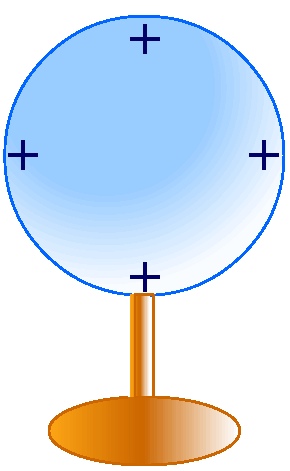
\includegraphics[width=0.15\textwidth]{src/coulombtheorem/image3.pdf}
          \end{figure}
    \item Il \textbf{campo elettrico all'interno di un conduttore è nullo} \ref{eq:gausslaw4}:\\
          \begin{equation}
              \boxed{\vec{E} = 0}
          \end{equation}
    \item Il conduttore \textbf{scherma} il \textbf{suo interno} da campi elettrici esterni.
          \begin{figure}[H]
              \centering
              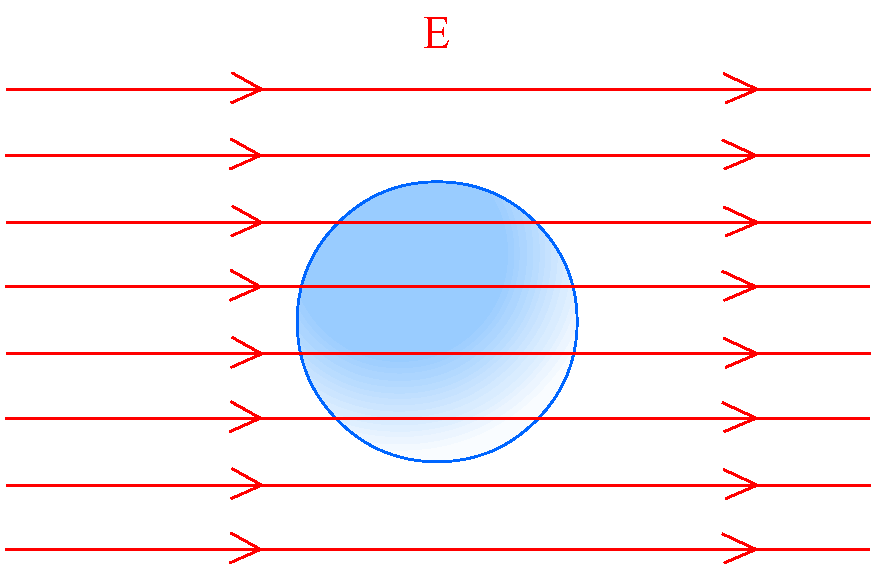
\includegraphics[width=0.30\textwidth]{src/coulombtheorem/image4.pdf}
              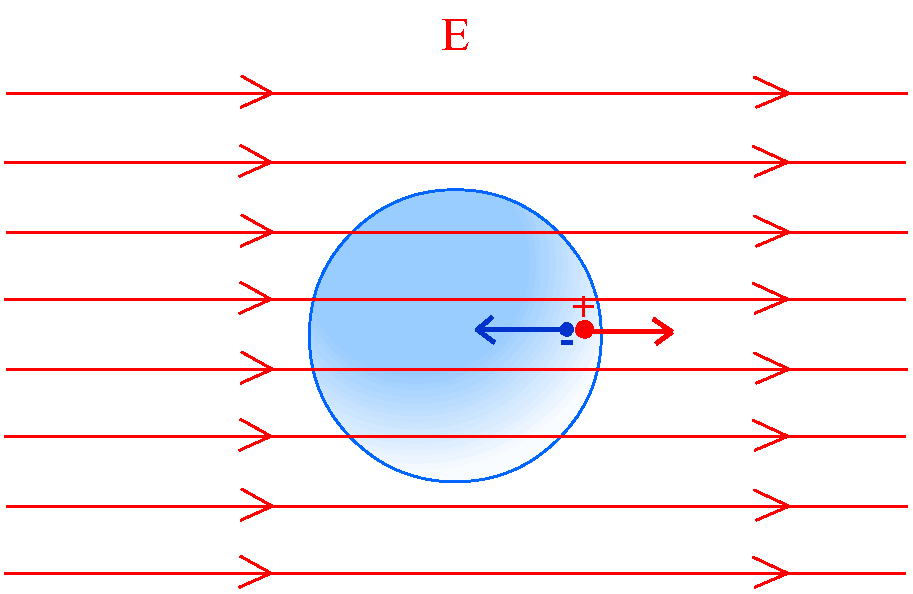
\includegraphics[width=0.30\textwidth]{src/coulombtheorem/image5.pdf}
              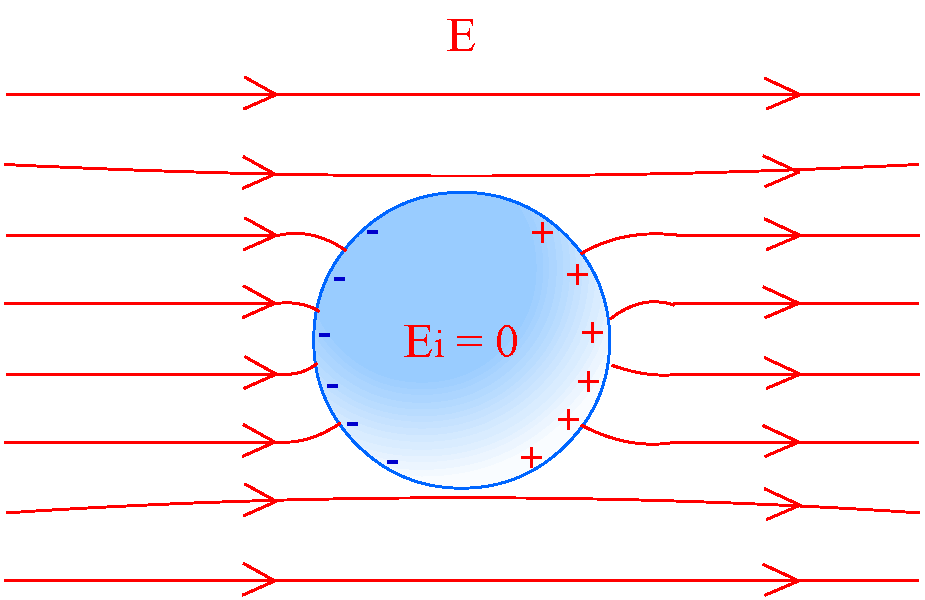
\includegraphics[width=0.30\textwidth]{src/coulombtheorem/image6.pdf}
          \end{figure}
          Non è banale il fatto schermi solo il suo interno,
          \begin{figure}[H]
              \centering
              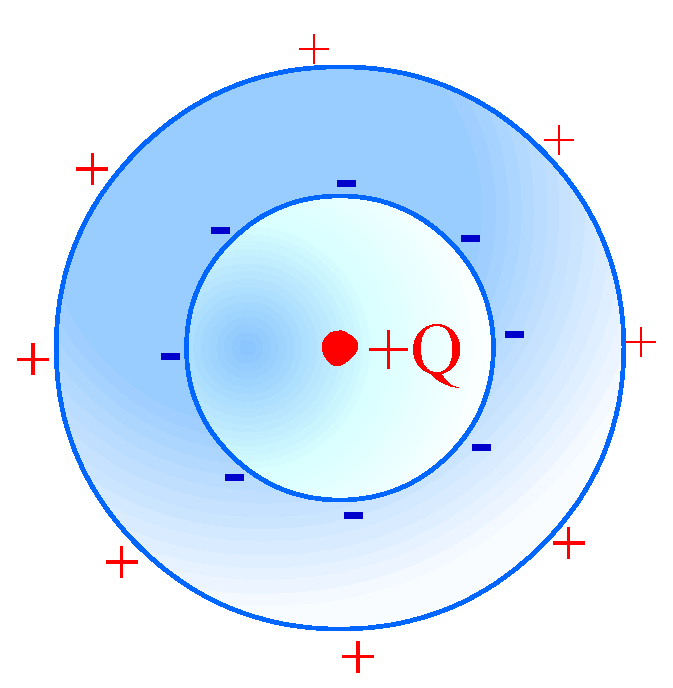
\includegraphics[width=0.30\textwidth]{src/coulombtheorem/image7.pdf}
              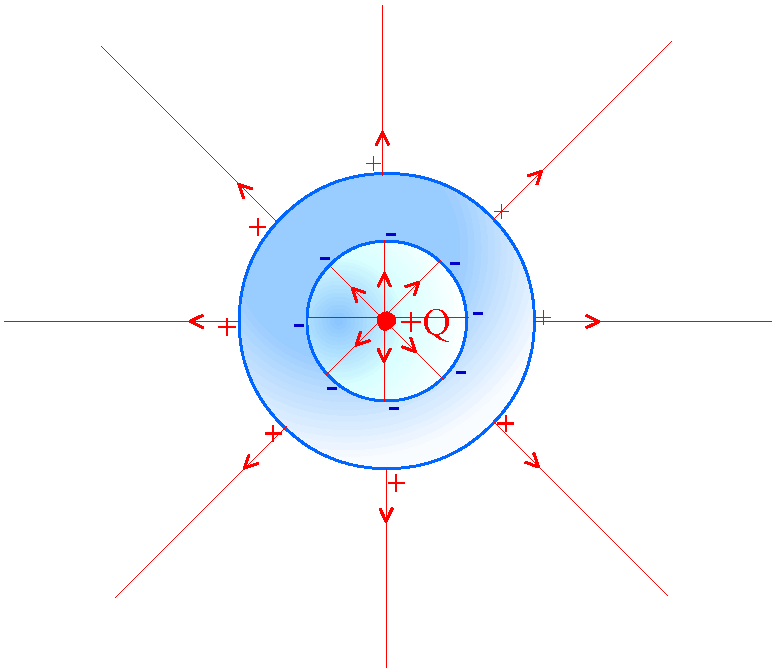
\includegraphics[width=0.30\textwidth]{src/coulombtheorem/image8.pdf}
          \end{figure}
\end{itemize}
\newpage
\subsection{Formule utili}
\textbf{Flusso del campo elettrico attraverso una superficie}
\begin{equation}
    \boxed{\Phi_{\vec{E}} = \displaystyle \int_{S} \vec{E} \cdot d\vec{S}}
\end{equation}
\textbf{Flusso del campo elettrico che attraversa una corpo chiuso}
\begin{equation}
    \boxed{\Phi_{\vec{E}} = 0}
\end{equation}
\textbf{Legge di Gauss}
\begin{equation}
    \boxed{\Phi_{\vec{E}} = \displaystyle \oint_S \vec{E} \cdot d\vec{S}}
\end{equation}
\begin{equation}
    \boxed{\Phi_{\vec{E}} = \displaystyle \frac{1}{\varepsilon_0} \sum_{i=1}^{n} q_{i}^{int}}
\end{equation}
\textbf{Campo elettrostatico di situazioni note}
\begin{itemize}
    \item Campo elettrostatico interno ed esterno ad un guscio carico sottile (2D)
          \begin{enumerate}
              \item Esterno del guscio
                    \begin{equation}
                        \boxed{\vec{E} = \displaystyle \frac{Q}{4\pi \varepsilon_0 r_{1}^2}}
                    \end{equation}
              \item Interno del guscio
                    \begin{equation}
                        \boxed{\vec{E} = 0}
                    \end{equation}
          \end{enumerate}
    \item Campo elettrostatico interno ed esterno ad una sfera uniformemente carica (3D)
          \begin{enumerate}
              \item Esterno della sfera
                    \begin{equation}
                        \boxed{\vec{E} = \displaystyle \frac{Q}{4\pi \varepsilon_0 r^2}}
                    \end{equation}
              \item Interno della sfera
                    \begin{equation}
                        \boxed{\vec{E} = \displaystyle \frac{Q}{4\pi \varepsilon_0 R^3} \cdot r}
                    \end{equation}
          \end{enumerate}
\end{itemize}
\textbf{Teorema di Coulomb}\\
In un conduttore
\begin{equation}
    \boxed{E = \displaystyle \frac{\sigma}{\varepsilon_0}}
\end{equation}
\begin{equation}
    \boxed{E = 0}
\end{equation}

\newpage
\section{Potenziale elettrico}
\subsection{Potenziale elettrostatico}
Remember :
\begin{itemize}
    \item \textbf{Lavoro} è l'energia trasferita da una forza ad un corpo in movimento.
    \item \textbf{Energia potenziale} è l'energia che un corpo possiede in virtù della sua posizione nello spazio, solo se la forza è conservativa.
\end{itemize}
Poiché la forza elettrostatica è conservativa, anche il campo elettrostatico è conservativo.\\
\begin{equation*}
    \mathcal{L}_{AB} = \displaystyle \int_{A}^{B} \vec{F} \cdot d\vec{r}
\end{equation*}
\begin{equation*}
    \mathcal{L}_{AB} = \displaystyle \int_{A}^{B} q \vec{E} \cdot d\vec{r}
\end{equation*}
\begin{equation*}
    \mathcal{L}_{AB} = q \displaystyle \int_{A}^{B} \vec{E} \cdot d\vec{r}
\end{equation*}
\begin{equation*}
    \mathcal{L}_{AB} = q \displaystyle \int_{A}^{B} \frac{Q}{4\pi \varepsilon_0 r^2} \cdot dr
\end{equation*}
\begin{equation*}
    \mathcal{L}_{AB} = \frac{qQ}{4\pi \varepsilon_0} \displaystyle \int_{A}^{B} \frac{1}{r^2} \cdot dr
\end{equation*}
\begin{equation*}
    \mathcal{L}_{AB} = \frac{qQ}{4\pi \varepsilon_0} \displaystyle \int_{A}^{B} r^{-2} \cdot dr
\end{equation*}
\begin{equation*}
    \mathcal{L}_{AB} = \frac{qQ}{4\pi \varepsilon_0} \displaystyle \int_{A}^{B} r^{-2} \cdot dr
\end{equation*}
\begin{equation*}
    \mathcal{L}_{AB} = \frac{qQ}{4\pi \varepsilon_0} \displaystyle \left[\frac{r^{-1}}{-1} \right]_{A}^{B}
\end{equation*}
\begin{equation*}
    \mathcal{L}_{AB} = \frac{qQ}{4\pi \varepsilon_0} \displaystyle \left[-\frac{1}{r} \right]_{A}^{B}
\end{equation*}
\begin{equation*}
    \mathcal{L}_{AB} = \frac{qQ}{4\pi \varepsilon_0} \displaystyle\left[ -\frac{1}{r_{B}} + \frac{1}{r_{A}}\right]
\end{equation*}
\begin{equation*}
    \mathcal{L}_{AB} = \frac{qQ}{4\pi \varepsilon_0} \displaystyle\left[ \frac{1}{r_{A}} - \frac{1}{r_{B}}\right]
\end{equation*}
Il lavoro dipende solo dalla posizione iniziale e finale, non dal percorso.\\
\begin{equation}
    \boxed{\mathcal{L} = \oint \vec{F} \cdot d\vec{l} = 0}
\end{equation}
\begin{equation}
    \boxed{\mathcal{L} = q\ \oint \vec{E} \cdot d\vec{l} = 0}
\end{equation}
\subsubsection{Energia potenziale elettrostostatica U}
Poiché la forza elettrostatica è conservativa, posso definire una funzione \(U(\vec{r})\) definita \textbf{energia potenziale elettrostatica} tale che
\begin{equation}
    \boxed{\Delta U = -\mathcal{L}_{AB}}
\end{equation}
\begin{equation*}
    U_B - U_A = - \displaystyle \int_{A}^{B} \vec{F} \cdot d\vec{r}
\end{equation*}
\begin{equation*}
    U_B - U_A = -\frac{qQ}{4\pi \varepsilon_0} \displaystyle\left[ \frac{1}{r_{A}} - \frac{1}{r_{B}}\right]
\end{equation*}
\begin{equation*}
    U_B - U_A = \frac{qQ}{4\pi \varepsilon_0} \displaystyle\left[ \frac{1}{r_{B}} - \frac{1}{r_{A}}\right]
\end{equation*}
\textbf{Energia potenziale elettrostatica di una carica puntiforme}\\
\noindent
Faccio un trick algebrico per trovare \(U_B\), l'energia potenziale di una carica \(q\) posta in un punto \(B\) distante \(r_B\) da \(Q\).\\
Faccio finta di partire da lontano \(A = r_{\infty}\) e arrivare a \(B = r_{B}\).
\begin{equation*}
    U_B - U_A = -\frac{qQ}{4\pi \varepsilon_0} \displaystyle\left[ \frac{1}{r_{A}} - \frac{1}{r_{B}}\right]
\end{equation*}
\begin{equation*}
    U_B - U_{\infty} = -\frac{qQ}{4\pi \varepsilon_0} \displaystyle\left[ \frac{1}{r_{\infty}} - \frac{1}{r_{B}}\right]
\end{equation*}
\begin{equation*}
    U_B - 0 = -\frac{qQ}{4\pi \varepsilon_0} \displaystyle\left[ 0 - \frac{1}{r_{B}}\right]
\end{equation*}
\begin{equation*}
    \boxed{U_B = \frac{qQ}{4\pi \varepsilon_0 r_{B}}}
\end{equation*}
\subsubsection{Potenziale elettrostatico V (o Tensione)}
Definisco il \textbf{potenziale elettrostatico} \(V\) come il rapporto tra l'energia potenziale elettrostatica \(U\) e la carica di prova \(q\).
\begin{equation*}
    V = \displaystyle \frac{U}{q}
\end{equation*}
\begin{equation*}
    V = \displaystyle \frac{1}{q} \cdot \frac{qQ}{4\pi \varepsilon_0 r}
\end{equation*}
\begin{equation}
    \boxed{V = \displaystyle \frac{Q}{4\pi \varepsilon_0 r}}
\end{equation}
\begin{equation*}
    \quad \left[V\right] = \frac{\left[J\right]}{\left[C\right]}\ \left[\text{Volt}\right] = \frac{\left[\text{Joule}\right]}{\left[\text{Coulomb}\right]}
\end{equation*}
\textbf{Note:}
\begin{itemize}
    \item Dipende solo dalla carica \(Q\) e dalla distanza \(r\).
    \item La carica di prova \textcolor{red}{\(+q\)} tende a muoversi da un punto di potenziale maggiore ad uno di potenziale minore.(il contrario se \textcolor{blue}{\(-q\)})
    \item Un altro nome per il potenziale elettrostatico è \textbf{tensione elettrostatica} o \textbf{tensione}.
\end{itemize}
\subsubsection{Relazione tra Campo elettrostatico (E) e potenziale elettrostatico (V)}
Partiamo dalla relazione tra \(U\) di un punto e \(F\)

\begin{multicols}{3}
    \noindent
    \begin{equation*}
        dU = -\vec{F} \cdot d\vec{r}
    \end{equation*}
    \columnbreak
    \noindent
    \begin{equation*}
        dU = q\ dV
    \end{equation*}
    \columnbreak
    \noindent
    \begin{equation*}
        \vec{F} = q\ \vec{E}
    \end{equation*}
\end{multicols}
\begin{equation}
    \boxed{dV = -\vec{E} \cdot d\vec{r}}
\end{equation}
\begin{equation*}
    \underbrace{dV} = \underbrace{-\vec{E} \cdot d\vec{r}}
\end{equation*}
\begin{equation*}
    \frac{\delta V}{\delta x} dx + \frac{\delta V}{\delta y} dy + \frac{\delta V}{\delta z} dz = -E_x dx - E_y dy - E_z dz
\end{equation*}
Per questo il campo elettrostatico \(\vec{E}\) ha come unità di misura
\begin{equation*}
    \vec{E} = \frac{\left[V\right]}{\left[m\right]} = \frac{\left[\text{Volt}\right]}{\left[\text{Metro}\right]} \quad \lor \quad \frac{\left[N\right]}{\left[C\right]} = \frac{\left[\text{Newton}\right]}{\left[\text{Coulomb}\right]}
\end{equation*}
Differenza di potenziale tra due punti \(A\) e \(B\) è :
\begin{equation*}
    \Delta V = V_B - V_A
\end{equation*}
\begin{equation*}
    \Delta V = -\displaystyle \int_{A}^{B} dV
\end{equation*}
\begin{equation}
    \boxed{\Delta V = -\displaystyle \int_{A}^{B} \vec{E} \cdot d\vec{r}}
\end{equation}
\begin{equation*}
    \boxed{\Delta V = -\vec{E} \int_{A}^{B} d\vec{r}}
\end{equation*}

\subsubsection{Potenziale elettrostatico V e distribuzione di carica continua}
\begin{equation*}
    dV = \displaystyle \frac{dq}{4\pi \varepsilon_0 r}
\end{equation*}
\begin{equation*}
    V = \displaystyle \int dV
\end{equation*}
\begin{equation*}
    \begin{cases}
        dV = \displaystyle \frac{\lambda dl}{4\pi \varepsilon_0 r} \\
        \\
        dV = \displaystyle \frac{\sigma dS}{4\pi \varepsilon_0 r}  \\
        \\
        dV = \displaystyle \frac{\rho dV}{4\pi \varepsilon_0 r}    \\
    \end{cases}
\end{equation*}

\subsubsection{Effetto delle punte}
Sui conduttori la carica si accumula maggiormente sulle punte.\\
\begin{figure}[H]
    \centering
    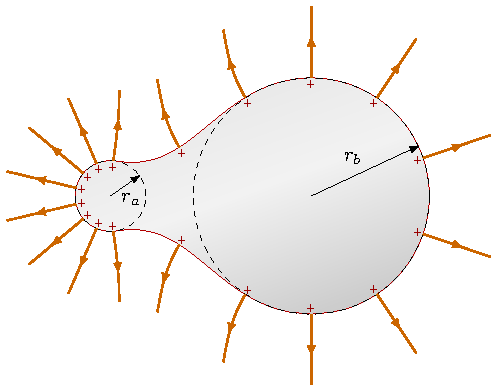
\includegraphics[width=0.40\textwidth]{src/electricfieldvolume/image2.pdf}
    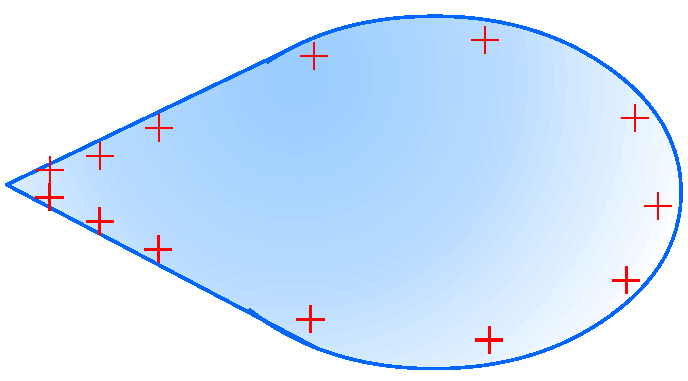
\includegraphics[width=0.35\textwidth]{src/coulombtheorem/image9.pdf}
\end{figure}
\subsection{Esempi vari}
\subsubsection{Es : Calcolare la differenza di potenziale tra P e un piano infinito carico con densità di carica superficiale}
Dalla relazione tra campo elettrico e potenziale elettrico
\begin{equation*}
    \Delta V = -\displaystyle \int_{A}^{B} \vec{E} \cdot d\vec{r}
\end{equation*}
\begin{equation*}
    V_P-V_O = -\displaystyle \int_{O}^{P} \frac{\sigma}{2 \varepsilon_0} \cdot d\vec{r}
\end{equation*}
\begin{equation*}
    V_P-V_O = -\frac{\sigma}{2 \varepsilon_0} \displaystyle \int_{O}^{P}  d\vec{r}
\end{equation*}
\begin{equation*}
    V_P-V_O = -\frac{\sigma}{2 \varepsilon_0}r
\end{equation*}
\begin{equation}
    \boxed{\Delta V = -\frac{\sigma}{2 \varepsilon_0}r}
\end{equation}
\subsubsection{Es : Calcolare la differenza di potenziale tra due armature con densità di carica superficiale}
\begin{equation}
    \boxed{\Delta V = \displaystyle \frac{|\sigma|}{\varepsilon_0} \cdot r}
\end{equation}
\newpage
\subsection{Formule utili}
\noindent
\textbf{Energia potenziale elettrostatica U}\\
Definzione
\begin{equation}
    \boxed{\Delta U = -\mathcal{L}_{AB}}
\end{equation}
In un punto (trick algebrico)
\begin{equation}
    \boxed{U_P = \displaystyle \frac{qQ}{4\pi \varepsilon_0 r_{P}}}
\end{equation}
\textbf{Potenziale elettrostatico V (o Tensione)}\\
\noindent
Definizione
\begin{equation}
    \boxed{V_P = \frac{U_P}{q}}
\end{equation}
In un punto
\begin{equation}
    \boxed{V_P = \displaystyle \frac{Q}{4\pi \varepsilon_0 r_P}}
\end{equation}
Si misura in Volt \(\left[V\right] = \frac{\left[J\right]}{\left[C\right]}\)\\
\noindent
\textbf{Relazione tra Campo elettrostatico (E) e potenziale elettrostatico (V)}
\begin{equation}
    \boxed{dV = -\vec{E} \cdot d\vec{r}}
\end{equation}
\begin{equation}
    \boxed{\Delta V = - \int_{A}^{B}\vec{E}\ d\vec{r}}
\end{equation}
\textbf{Potenziale elettrostatico V e distribuzione di carica continua}
\begin{equation}
    \boxed{dV = \displaystyle \frac{ dq }{4\pi \varepsilon_0 r}}
\end{equation}
\begin{equation}
    \boxed{V = \displaystyle \int dV}
\end{equation}

\newpage
\section{Capacità elettrica e dielettrici}
\subsection{Capacità elettrica di un conduttore}
\begin{equation}
    \boxed{C = \displaystyle \frac{Q}{\Delta V}}
\end{equation}
L'unità di misura è
\begin{equation*}
    C = \left[\text{Farad}\right] = \frac{\left[\text{Coulomb}\right]}{\left[\text{Volt}\right]}
\end{equation*}
\subsection{Momento di dipolo elettrico}
\begin{equation}
    \boxed{\vec{p} = q \cdot \vec{d}}
\end{equation}
\subsubsection{Momento torcente su un dipolo elettrico in un campo elettrico}
\begin{equation}
    \boxed{\vec{\tau} = \vec{F} \times \vec{r}}
\end{equation}
\begin{equation}
    \boxed{\vec{\tau} = \vec{p} \times \vec{E}}
\end{equation}


\end{document}